% A LaTeX template for MSc Thesis submissions to 
% Politecnico di Milano (PoliMi) - School of Industrial and Information Engineering
%
% S. Bonetti, A. Gruttadauria, G. Mescolini, A. Zingaro
% e-mail: template-tesi-ingind@polimi.it
%
% Last Revision: October 2021
%
% Copyright 2021 Politecnico di Milano, Italy. NC-BY

\documentclass{Configuration_Files/PoliMi3i_thesis}

%------------------------------------------------------------------------------
%	REQUIRED PACKAGES AND  CONFIGURATIONS
%------------------------------------------------------------------------------

% CONFIGURATIONS
\usepackage{parskip} % For paragraph layout
\usepackage{setspace} % For using single or double spacing
\usepackage{emptypage} % To insert empty pages
\usepackage{multicol} % To write in multiple columns (executive summary)
\setlength\columnsep{15pt} % Column separation in executive summary
\setlength\parindent{0pt} % Indentation
\raggedbottom  

% PACKAGES FOR TITLES
\usepackage{titlesec}
% \titlespacing{\section}{left spacing}{before spacing}{after spacing}
\titlespacing{\section}{0pt}{3.3ex}{2ex}
\titlespacing{\subsection}{0pt}{3.3ex}{1.65ex}
\titlespacing{\subsubsection}{0pt}{3.3ex}{1ex}
\usepackage{color}

% PACKAGES FOR LANGUAGE AND FONT
\usepackage[english]{babel} % The document is in English  
\usepackage[utf8]{inputenc} % UTF8 encoding
\usepackage[T1]{fontenc} % Font encoding
\usepackage[11pt]{moresize} % Big fonts

% PACKAGES FOR IMAGES
\usepackage{graphicx}
\usepackage{transparent} % Enables transparent images
\usepackage{eso-pic} % For the background picture on the title page
\usepackage{subfig} % Numbered and caption subfigures using \subfloat.
\usepackage{tikz} % A package for high-quality hand-made figures.
\usetikzlibrary{}
\graphicspath{{./Images/}} % Directory of the images
\usepackage{caption} % Coloured captions
\usepackage{xcolor} % Coloured captions
\usepackage{amsthm,thmtools,xcolor} % Coloured "Theorem"
\usepackage{float}

% STANDARD MATH PACKAGES
\usepackage{amsmath}
\usepackage{amsthm}
\usepackage{amssymb}
\usepackage{amsfonts}
\usepackage{bm}
\usepackage[overload]{empheq} % For braced-style systems of equations.
\usepackage{fix-cm} % To override original LaTeX restrictions on sizes

% PACKAGES FOR TABLES
\usepackage{tabularx}
\usepackage{longtable} % Tables that can span several pages
\usepackage{colortbl}

% PACKAGES FOR ALGORITHMS (PSEUDO-CODE)
\usepackage{algorithm}
\usepackage{algorithmic}

% PACKAGES FOR REFERENCES & BIBLIOGRAPHY
\usepackage[colorlinks=true,linkcolor=black,anchorcolor=black,citecolor=black,filecolor=black,menucolor=black,runcolor=black,urlcolor=black]{hyperref} % Adds clickable links at references
\usepackage{cleveref}
\usepackage[square, numbers, sort&compress]{natbib} % Square brackets, citing references with numbers, citations sorted by appearance in the text and compressed
\bibliographystyle{unsrt} % You may use a different style adapted to your field
% \bibliographystyle{ieeert}

% OTHER PACKAGES
\usepackage{pdfpages} % To include a pdf file
\usepackage{afterpage}
\usepackage{lipsum} % DUMMY PACKAGE
\usepackage{fancyhdr} % For the headers
\fancyhf{}

% Input of configuration file. Do not change config.tex file unless you really know what you are doing. 
\input{Configuration_Files/config}


%----------------------------------------------------------------------------
%	NEW COMMANDS DEFINED
%----------------------------------------------------------------------------

% EXAMPLES OF NEW COMMANDS
\newcommand{\bea}{\begin{eqnarray}} % Shortcut for equation arrays
\newcommand{\eea}{\end{eqnarray}}
\newcommand{\e}[1]{\times 10^{#1}}  % Powers of 10 notation
\newcommand{\mathbbm}[1]{\text{\usefont{U}{bbm}{m}{n}#1}} % From mathbbm.sty

\newcommand{\etal}{\textit{et al}., }
\newcommand{\ie}{\textit{i}.\textit{e}., }
\newcommand{\eg}{\textit{e}.\textit{g}.\ }
\newcommand{\wrt}{\textit{w}.\textit{r}.\textit{t}.\ }

%----------------------------------------------------------------------------
%	ADD YOUR PACKAGES (be careful of package interaction)
%----------------------------------------------------------------------------
\usepackage{easyReview}
\usepackage[utf8]{inputenc}
\usepackage[acronym, nomain]{glossaries}
\makeglossaries
\usepackage{mathtools}

%----------------------------------------------------------------------------
%	ADD YOUR DEFINITIONS AND COMMANDS (be careful of existing commands)
%----------------------------------------------------------------------------

%----------------------------------------------------------------------------
%	BEGIN OF YOUR DOCUMENT
%----------------------------------------------------------------------------

\begin{document}

\fancypagestyle{plain}{%
\fancyhf{} % Clear all header and footer fields
\fancyhead[RO,RE]{\thepage} %RO=right odd, RE=right even
\renewcommand{\headrulewidth}{0pt}
\renewcommand{\footrulewidth}{0pt}}
\newacronym{3GPP}{3GPP}{3rd Generation Partnership Project}
\newacronym{5G}{5G}{fifth generation}
\newacronym{6G}{6G}{sixth generation}
\newacronym{ai}{AI}{artificial intelligence}
\newacronym{aoa}{AOA}{angle of arrival}
\newacronym{awgn}{AWGN}{additive white Gaussian noise}
\newacronym{bts}{BTS}{base transceiver station}
\newacronym{cacfar}{CA-CFAR}{cell-averaging CFAR}
\newacronym{cdf}{CDF}{cumulative distribution function}
\newacronym{cid}{CID}{cell ID}
\newacronym{cfar}{CFAR}{constant false alarm rate}
\newacronym{cp}{CP}{cyclic prefix}
\newacronym{cran}{C-RAN}{centralised radio access network}
\newacronym{csi}{CSI}{channel state information}
\newacronym{cu}{CU}{centalised unit}
\newacronym{cut}{CUT}{cell under test}
\newacronym{dl}{DL}{downlink}
\newacronym{dfs}{DFS}{discrete Fourier series}
\newacronym{dft}{DFT}{discrete Fourier transform}
\newacronym{du}{DU}{distributed unit}
\newacronym{fft}{FFT}{Fast Fourier Transform}
\newacronym{fmcw}{FMCW}{frequency modulated continous wave}
\newacronym{fr1}{FR1}{frequency range 1}
\newacronym{fr2}{FR2}{frequency range 2}
\newacronym{fr3}{FR3}{frequency range 3}
\newacronym{GNSS}{GNSS}{Global Navigation Satellite System}
\newacronym{gnb}{gNB}{gNodeB}
\newacronym{idft}{IDFT}{inverse discrete Fourier transform}
\newacronym{ifft}{iFFT}{inverse Fast Fourier Transform}
\newacronym{iot}{IoT}{Internet of Things}
\newacronym{isac}{ISAC}{Integrated Sensing and Communication}
\newacronym{isi}{ISI}{inter-symbol interference}
\newacronym{kf}{KF}{Kalman filter}
\newacronym{los}{LOS}{line of sight}
\newacronym{lte}{LTE}{long-term evolution}
\newacronym{map}{MAP}{maximum a posteriori}
\newacronym{mimo}{MIMO}{multiple input multiple output}
\newacronym{ml}{ML}{machine learning}
\newacronym{nlos}{NLOS}{non-line of sight}
\newacronym{NR}{NR}{New Radio}
\newacronym{ofdm}{OFDM}{Orthogonal Frequency Division Multiplexing}
\newacronym{otfs}{OTFS}{Orthogonal Time Frequency Space}
\newacronym{papr}{PAPR}{peak-to-average power ratio}
\newacronym{pdf}{PDF}{probability density function}
\newacronym{pg}{PG}{processing gain}
\newacronym{phy}{PHY}{physical layer}
\newacronym{poc}{PoC}{proof of concept}
\newacronym{psd}{PSD}{power spectral density}
\newacronym{psf}{PSF}{point-spread function}
\newacronym{ru}{RU}{radio unit}
\newacronym{rcs}{RCS}{radar cross section}
\newacronym{snr}{SNR}{signal-to-noise ratio}
\newacronym{spu}{SPU}{sensing processing unit}
\newacronym{tdd}{TDD}{time division duplexing}
\newacronym{toa}{TOA}{time of arrival}
\newacronym{uav}{UAV}{unmanned aerial vehicles}
\newacronym{ue}{UE}{User Equipment}
\newacronym{ul}{UL}{uplink}
\newacronym{v2x}{V2X}{vehicle-to-everything}
\newacronym{wosa}{WOSA}{window-overlap spectral analysis}
%----------------------------------------------------------------------------
%	TITLE PAGE
%----------------------------------------------------------------------------

\pagestyle{empty} % No page numbers
\frontmatter % Use roman page numbering style (i, ii, iii, iv...) for the preamble pages

\puttitle{
	title=Feasibility of Non-Line of Sight \newline Integrated Sensing and \newline Communication at mmWave, % Title of the thesis
	name=Paolo Tosi, % Author Name and Surname
	course=Telecommunications Engineering - Ingegneria delle Telecomunicazioni, % Study Programme (in Italian)
	ID  = 997038,  % Student ID number (numero di matricola)
	advisor= Prof. Maurizio Magarini, % Supervisor name
	coadvisor={Marcus Henninger, Dr. Silvio Mandelli}, % Co-Supervisor name, remove this line if there is none
	academicyear={2023-24},  % Academic Year
} % These info will be put into your Title page 

%----------------------------------------------------------------------------
%	PREAMBLE PAGES: ABSTRACT (inglese e italiano), EXECUTIVE SUMMARY
%----------------------------------------------------------------------------
\startpreamble
\setcounter{page}{1} % Set page counter to 1

% ABSTRACT IN ENGLISH
\chapter*{Abstract} 

One of the new key features behind the development of sixth-generation (6G) mobile networks is their ability to gather information about the surrounding environment. 
Orthogonal Frequency Division Multiplexing (OFDM) radio signals, which are transmitted by base stations to users and vice versa, not only carry data, but are also affected by the movement of the transmitter, obstacles, and illuminated targets.
The concept of OFDM radar aims to extract information about the distance and relative speeds of targets that reflect the signal.
The high bandwidths and large antenna apertures available in next-generation mobile networks will facilitate the usage of OFDM radar for gathering sensing information. 
The combination of these functions and the underlying existing communication capabilities is referred to as Integrated Sensing and Communication (ISAC).
Applications typically considered for ISAC include vehicle detection (cars or drones), human activity detection and industrial safety. 
The typical assumption is that the target is in \gls{los} from the sensing hardware. 
However, an area that has not been extensively explored is non-line-of-sight (NLOS) sensing, where the radio signal can, if at all, reach the target after multiple reflections.
The aim of this thesis work is to investigate the feasibility of ISAC in NLOS environments, addressing performance constraints imposed by communication requirements, algorithmic development and identification of novel application scenarios for the system.
The proposed approaches are validated using real-world measurements obtained from Nokia's ISAC mmWave prototype, which was deployed in an industrial test facility in the ARENA 2036 in Stuttgart, Germany.
The prototype is based on a commercial system that operates at 27.4 GHz and complies with the 3rd Generation Partnership Project (3GPP) standards for fifth-generation (5G) waveforms in the mmWave frequency bands. 
% The system is extended by an additional radio unit called 'Sniffer' for receiving signals reflected by the target, and a 'Sensing Processing Unit (SPU)' which is responsible for performing the radar processing algorithms.
Validation measurements were performed focusing on human intrusion detection scenarios in an industrial environment.
The objective is to define an initial approach for NLOS radar sensing based on periodogram spectral analysis, which can be exploited for more advanced sensing functionalities.
\\
\\
\textbf{Keywords:} ISAC, 6G, OFDM radar, monostatic sensing, non-line-of-sight sensing % Keywords

% ABSTRACT IN ITALIAN
\chapter*{Abstract in lingua italiana}
Lo sviluppo delle reti mobili di sesta generazione (6G) è incentrato sulla capacità di raccogliere informazioni sull'ambiente circostante.
I segnali radio a divisione di frequenza ortogonale (OFDM), che vengono trasmessi dalle stazioni base agli utenti e viceversa, non solo trasportano dati, essi sono influenzati dal movimento del trasmettitore, dagli ostacoli e dai soggetti illuminati dal segnale.
Il concetto di radar OFDM mira a estrarre informazioni sulla distanza e sulla velocità relativa dei bersagli analizzando il segnale riflesso.
Grazie all'elevata larghezza di banda disponibile nelle reti mobili di prossima generazione, il radar OFDM può essere implementato per ottenere informazioni con elevata precisione.
La combinazione di queste funzioni e delle capacità cellulari sottostanti
è denominata Integrated Sensing and Communications (ISAC). Le applicazioni tipicamente considerate per ISAC sono il rilevamento di veicoli (automobili o droni), il rilevamento di attività umane e la sicurezza industriale.
in questi casi d'uso si suppone che il bersaglio venga illuminato in linea diretta segnale radio, condizione denominata di \textit{line-of-sight} (\gls{los}). Tuttavia, un ambito non ancora esplorato in modo esaustivo è quello in cui il bersaglio non si trova in linea diretta, ma viene raggiunto dal segnale solo dopo riflessioni su altri ostacoli, condizione indicata come \textit{non-line-of-sight} (NLOS).
L'obiettivo di questo lavoro di tesi è studiare la fattibilità di sistemi ISAC in condizioni di NLOS, affrontando i vincoli sulle prestazioni imposti dai requisiti di comunicazione, dallo sviluppo di algoritmi e dall'identificazione di nuovi scenari applicativi per il sistema.
Gli approcci proposti sono stati convalidati utilizzando misure reali
ottenute dal prototipo ISAC mmWave di Nokia, installato in
una struttura di ricerca industriale ad ARENA 2036, Stoccarda, Germania. 
Il prototipo è basato su un sistema commerciale che opera a 27,4 GHz, conforme alle specifiche del 3rd Generation Partnership Project (3GPP) per le forme d'onda di quinta generazione (5G).
Le misurazioni sono state eseguite su scenari di rilevamento delle intrusioni umane in un ambiente industriale. 
L'obiettivo di questa tesi è quello di definire un primo approccio per il rilevamento radar in NLOS basato sull'analisi spettrale del periodogramma.
\\
\\
\textbf{Parole chiave:} ISAC, 6G, radar OFDM, radar monostatico, rilevamento NLOS % Keywords (italian)

%----------------------------------------------------------------------------
%	LIST OF CONTENTS/FIGURES/TABLES/SYMBOLS
%----------------------------------------------------------------------------

% TABLE OF CONTENTS
\thispagestyle{empty}
\tableofcontents % Table of contents 
\thispagestyle{empty}
\cleardoublepage

%-------------------------------------------------------------------------
%	THESIS MAIN TEXT
%-------------------------------------------------------------------------
% In the main text of your thesis you can write the chapters in two different ways:
%
%(1) As presented in this template you can write:
%    \chapter{Title of the chapter}
%    *body of the chapter*
%
%(2) You can write your chapter in a separated .tex file and then include it in the main file with the following command:
%    \chapter{Title of the chapter}
%    \input{chapter_file.tex}
%
% Especially for long thesis, we recommend you the second option.

\addtocontents{toc}{\vspace{2em}} % Add a gap in the Contents, for aesthetics
\mainmatter % Begin numeric (1,2,3...) page numbering

% --------------------------------------------------------------------------
% NUMBERED CHAPTERS % Regular chapters following
% --------------------------------------------------------------------------

% Template text from model, remove after starting to write
% \include{Template}

% Introduction
\chapter{Introduction}
\label{chap_intro}

Mobile cellular networks beyond fifth and sixth-generation wireless systems (5G and 6G) are set to provide connectivity not only to end-users with improved capabilities, but also to different types of devices such as buildings, vehicles, and appliances.
Although the focus of 5G is on connecting devices from the Internet of Things (IoT) and helping to automate industrial systems, 6G aims to unify the human experience across the physical, digital, and human world \cite{6G-explained-NOKIA}.

% TODO: search image from Thorsten's article

\begin{figure}[H]
    \centering
    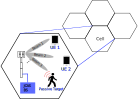
\includegraphics[width=0.7\textwidth]{Images/introduction/isac-scheme-1.png}
    \caption{Illustration of an ISAC scenario.}
    \label{fig:isac-scheme-1}
\end{figure}

6G will build on top of 5G and 5G-Advanced systems and use cases, driving their adoption through optimization and cost reduction. Nonetheless, new use-cases will be defined and enabled by the network's new abilities.

Thanks to the massive deployment of connected sensors and artificial intelligence (AI/ML) it will be possible to generate digital twins capable of real-time updates and prediction.  Digital twin models are essential for understanding what is occurring in the real world, predicting potential results, forecasting needs, and taking effective measures.

One of the most notable advancements in 6G technology will be the ability to perceive the surrounding environment, including people and objects, called network sensing. This capability converts the network into a source of valuable situational data by capturing and interpreting signals reflected by various entities. Determining characteristics such as type, shape, relative position, speed, and even material properties, advanced sensing empowers the creation of true-to-model digital twins. Moreover, when this data is fused with information from other sensors, artificial intelligence and machine learning, it unlocks new insights from the physical world, enhancing the network's cognitive abilities.

% TODO: add description of various chapters


% Overview of 6G sensing
\chapter{Overview of 6G ISAC}

The fifth generation of wireless communication systems introduced, with the 5G New Radio (NR), support for radio-access-technology-based localization, precise positioning protocol and the possibility of measuring gaps on the New Radio (NR) carrier. This enables the UE to estimate positions with time difference of arrival measurements \cite{Keating_Saily_Hulkkonen_Karjalainen_2019} . \newline
The NR positioning protocol can also integrate satellite-based positioning systems and can be deployed as a private network solution with active user localization as in \cite{Henninger_Abrudan_Mandelli_Arnold_Saur_Kolmonen_Klein_Schlitter_Brink_2022}.
The current standards, however, do not allow to detect passive devices, which refers to objects not directly connected to the network.

With the objective of expanding the capabilities of the mobile network, Integrated Sensing and Communication (also known as JCAS or ICAS) has been a topic of interest in the 6G research community \cite{Mandelli_Henninger_Bauhofer_Wild_2023}.

It is said that 6G will function as a network with a sixth sense \cite{Viswanathan_Wild_2021}. Radio signals transmitted by base stations, or users do not only carry data. They are effected by the movement of the transmitter or receiver, obstacles and illuminated objects' movement or changes in the propagation medium. Radio channels bear information about the environment in which the signal is transmitted. 
Channel information can be obtained by comparing the reflected signal with the known transmitted one. By analysing the channel response, it is possible to extract details about position, relative speed, type and shape of illuminated object.

For 6G, the RF sensing capabilities should be integrated in-band, using the same spectrum for both communication and radar sensing purposes. Figure \ref{fig:ISAC-scheme} illustrates a fundamental sketch of an ISAC scenario. In this depiction, a cellular system is shown with the presence of multi-cell interference. The system is equipped with array antennas capable of beamforming, serving the dual purpose of sensing and facilitating high-rate, low-latency communication to multiple users.

Integrated sensing and communications will benefit from the current massive deployment of cellular systems and their increasing density: making use of existing hardware and extending its capabilities with sensing could enable multi-user communication and multi-target detection with extended coverage



\section{Technological enablers}
	
	In recent years Radar and communication front-ends have become very similar, facilitating the integration of sensing and communication technology.
	Traditional radar systems were heavily reliant on hardware components to perform their core functions. However, with the advent of advanced digital technologies, a substantial number of these functions are now being realized through virtualization and digital signal processing. 

	This section will present some of the main technological aspects and digital technologies enabling joint functionality and the current research on RadCom systems.	
	
	\subsection{Spectrum choice for 6G sensing}
	
	% TODO: improve this
	One of the goals set for the sixth generation of wireless networks is to make efficient usage of the available spectrum which is the scarcest resource in communications.
	
	Future systems will probably make use of larger frequency bands, exploiting high bandwidth to perform high-resolution sensing. From 20 MHz carriers in LTE, 100 MHz and 400 MHz in respectively 5G NR and mmWave NR, it can be expected that 5G evolution and 6G systems will use bandwidths in the order of 1 GHz or more. A large usable bandwidth allows for increased sensing resolution, comparable to the one of an ad-hoc radar systems.
	
	Spectrum choice will be the determinant factor for the definition of overall capabilities of the system. The frequency ranges that are being considered for 6G \cite{Hexa} are:
	
	\begin{itemize}
		\item Frequency Range 1 (FR1): from 600 MHz to 6 GHz;
		\item Frequency Range 2 (FR2): mmWave, from 24 GHz to 71 GHz;
		\item the new Frequency Range 3 (FR3), not yet specified: from 7 to 20 GHz
	\end{itemize}
	
	Frequency range 1 is currently used for 5G capacity layers, providing bandwidth up to 100 MHz. For 6G, the main capacity layer will be placed in the "Golden Band" in 6-14 GHz, offering up to 400 MHz of bandwidth. FR2 in the millimetre frequency bands will start at 24 GHz and offer significantly more bandwidth, up to 800 MHz.
	
	Golden Band and FR2 are the most relevant candidates for defining the sensing spectrum in 6G. Their selection would make sense for wide area sensing and high resolution sensing respectively.
	
	Feasible use cases and possible scenarios will be driven by the characteristics and specifications offered by the frequency band of choice. It can be expected that FR2 will be used in micro-cellular deployments. They will be deployed in indoor environments, such as factory floors. Sensing targets in such environment will likely be pedestrians, passive factory objects and vehicles.
	Macro-cellular environments in the Golden Bands will dominate outdoors, where targets of interest will e vehicles for traffic monitoring, roadside safety and even detection of unmanned aerial vehicles (UAV) or drones.
	
	\subsection{Waveform candidates for ISAC}
	
	Waveform design is a fundamental building block of any radar or communication systems. Traditional radar and communication systems use waveforms optimized for the respective use, that are, in general, very different \cite{Zhang_Rahman_Wu_Huang_Guo_Chen_Yuan_2022}.
	
	In this work we refer to a communication-centric design, where the communication system is adapted and expanded in order to perform the sensing operation, sharing the main hardware and resources provided by the wireless mobile network.
	 
	
	\subsubsection{Traditional radar waveforms}
	
	Conventional radar systems mainly consist of pulsed and continuous wave radar. Both types can be further categorised according to whether the wave is modulated in frequency or phase \cite{Friedlander_2007}.
	Pulsed radar transmits short, typically unmodulated, pulses or bursts of pulses of large bandwidth, followed by a silent period, waiting for the reception of the echoed signal. Continuos wave radar are currently largely used in the automotive systems and the main example is the frequency modulated continuous wave (FMCW) radar. This systems transmit chirp signals with fixed or variable frequencies, which get shifted by the so called beat frequency when they get reflected by objects.
	
	Radar systems are typically designed to enable high power transmission with a relatively simple receiver structure. Two of the main design objectives are amplifier efficiency and ideal autocorrelation properties of the radar wave. Waveforms with low peak-to-average power ratio (PAPR) enable high efficiency and long range transmission.
	
	Due to their specialized signal shape and relatively simple hardware, this systems cannot support high data-rates for communication purposes, especially the ones that will be required by 6G.
	
	\subsubsection{Communication-centric waveforms}
	
	Current mobile communications are dominated by single-carrier and multi-carrier waveforms (OFDM).
	OFDM has become the current waveform reference in ISAC. Fully established in 4G and 5G communications systems, in the last decade it has also attracted the attention of the radar world.
	
	OFDM offers great multiplexing capabilities, both in time and in frequency, through the definition \textit{OFDM resource elements} that can be dynamically allocated to users. The use of cyclic prefix transforms the linear convolution of the signal with the channel response into a circular convolution, allowing convenient equalisation of the channel in the frequency domain \cite{Wild_Grudnitsky_Mandelli_Henninger_Guan_Schaich_2023}. In scenarios limited by PAPR constraints, such as uplink transmission, DFT spreading can  be applied on top of OFDM to achieve a single-carrier frequency division multiple access (SC-FDMA) scheme.
	
	Multicarrier waveforms offer the possibility of obtaining sensor information by using signal processing techniques that reduce the autocorrelation requirements required to radar waveforms \cite{Sturm_Wiesbeck_2011}.The main disadvantage of OFDM is the high peak to average power ratio (PAPR) and the additional DSP required for the joint communication and sensing data processing.
	
	\subsubsection{Waveforms for next-gen communication networks}
	
	A major challenge for OFDM and multi-carrier signals is their performance in highly frequency-dispersive channels. 
	The effect of phase noise and movement (Doppler spread) is enhanced at high carrier frequencies. 
	Due to the expansion of 5G and 6G systems towards mmWave, tackling this challenge is fundamental for ensuring high performance under these circumstances.
	
	Orthogonal time frequency space (OTFS) has been proposed as a modulation effective in tackling this problems \cite{OTFS_Hadani_2017}. OTFS operates in the delay-Doppler domain. 
	The fading, time-variant channel seen by an OFDM signal is transformed into a non-fading, time-independent channel through a 2D Fourier transform. 
	Applying this transformation and equalization within this domain each symbol will experience similar gain during transmission.
	
	The Orthogonal Time Frequency Space (OTFS) modulation scheme can be interpreted as the sequence of two transformations. 
	Firstly, the transmitter maps the complex symbols into discrete slots of the NxM delay-Doppler domain.
	Secondly, these symbols are transformed in the time-frequency domain through a 2D inverse symplectic finite Fourier transform (iSFFT). The the time-domain signal is obtained by an M-point inverse Fourier transform (iFFT). 
	The receiver will perform the inverse operation using FFT and SFFT respectively.
	OTFS is an ideal waveform for integrating sensing and communication due to its inherent property of exploiting the delay-Doppler domain.
	This is because information about the surrounding environment is necessary for improving communication performance.
	
	Although OTFS has proved to achieve a 3-7 dB advantage compared to OFDM in highly fading and mobility scenarios, however its implementation in real systems is hindered by some open research problems \cite{Wei_Yuan_OTFS_whitepaper_2021}. 
	The primary challenge is to develop an efficient decoding method for OTFS symbols.
	The output signal in the delay-Doppler domain is 2D circular convolution of the transmitted data symbols and the channel response. Although optimal detectors, such as maximum a posteriori (MAP) detectors, can mitigate channel interference and perfectly retrieve the original symbols, but they are too complex and costly.
	
	This work will focus on Orthogonal Frequency Division Multiplexing (OFDM), as it is the waveform currently used in 5G systems and in the proof of concept by Nokia. 
	
	 
	
	\subsection{5G functional splits}
	
	A functional split determines the number of functions implemented locally at the antenna site and, consequently, the functions to be implemented in a centralised datacenter \cite{Larsen_Checko_Christiansen_2019}. 
 	This solution was developed to define a flexible approach to the centralised radio access network (C-RAN) concept, that could work with the high data rates expected in 5G. 
	In NR, the radio processing stack defined by 3GPP is split between a distributed unit (DU) and a centralised unit (CU). 
	The general idea is to keep functions close to the user in the DU, while placing more complex and computationally intensive functions in the CU. The CU is usually represented by powerful datacenters.
	Allocating more functions in the DU means less traffic on the fronthaul network, but requires more powerful and expensive hardware at the antenna site.
	 
	Functional splits allow for a fairly flexible architecture of the system. Additional functionality, such as network sensing, can be implemented at the antenna site by adding dedicated processing hardware.

	\begin{figure}[H]
		\centering
		\includegraphics[width=0.5\textwidth]{Images/overview/5Gsplits_Larsen.png}
		\caption{Scheme representing the LTE protocol stack, showing proposed functional splits \cite{Larsen_Checko_Christiansen_2019}. }
		\label{fig:Overview-LTE_stack_splits}
	\end{figure}
	 
	
	\subsection{Massive MIMO and digital beamforming}
	
	Massive MIMO and digital beamforming can set the basis for performing high-resolution three-dimensional scans of the surrounding environment \cite{MIMO-next-gen}.
	The general idea is to intelligently combine the signals received from multiple antennas to achieve the best signal-to-noise ratio and the highest data rate. The signal combination is performed in the digital domain, after conversion to baseband, which offers the possibility of applying a variety of algorithms.
	
	In 5G, beamforming commonly employs an all-digital approach at lower frequencies. However, for mmWave frequencies and above, digitally controlled analogue or hybrid beamforming is typically used. In the hybrid approach one beam gets scanned at a time. A beam sweep can be performed by the transmitting cells, and the procedure of computing the range-Doppler profile of all beams in a cell is referred to as beam sweep. A similar procedure to a beam sweep is already used in 5G NR for synchronization signalling \cite{Wild_Braun_Viswanathan_2021}.
	
	\subsection{Signal processing enhanced by AI/ML}
	Generally, radar returns provide additional information beyond the range-Doppler profile. By analysing the channel information, it may be possible to extract target characteristics such as radar cross-section, micro-Doppler information, or the object's material or shape.
	This additional information can be used to solve a classification problem of objects and returns detected in the radar datacube.
	
	In recent years


\section{Proof of concept architecture}
	\label{sec:intro-PoCarchitecture}
	
	One of the objectives of ISAC is to make the best use of the deployed communication hardware to perform sensing. 
	The architecture considered in this work is based on a FR2 5G commercial communication hardware.
	
	Using option 7-2 of the proposed 5G splits, shown in Figure \ref{fig:Overview-LTE_stack_splits}, it is possible to use the same type of Remote Unit (RU) for both communication and sensing.
	Option 7-2 splits the network at the physical layer (PHY) level, which handles the conversion of digital data to the analogue radio signal in the downlink (DL) direction, while doing the opposite in the uplink (UL) direction.
	This split defines the FFT/iFFT performed in the RU, while the frequency domain IQ is transported on the fronthaul.
	The gNB RU operates in time-division duplexing (TDD) mode, where uplink is separated from downlink by the allocation of different time slots in the same frequency band. 	
	The sniffer operates always in uplink (UL) mode, receiving both the signal transmitted by UEs and the reflected signals. 
	
	The system is extended by an additional RU called \textit{Sniffer} and a server called \textit{Sensing Processing Unit} (SPU). 
	The sniffer is synchronized with the gNB by the same synchronization source. 
	The SPU receives the complex IQ signal (on a per-radio frame basis),  after removal of the cyclic prefix (CP), as input for further sensing processing \cite{Wild_Grudnitsky_Mandelli_Henninger_Guan_Schaich_2023}.
	
	This work considers a PoC deployment where the primary gNB RU and the sniffer are mounted in proximity and are co-located, allowing the system to behave as a monostatic radar. 
	The scope of this work does not cover the case of bistatic radar.
	
	The SPU processing chain for sensing is structured as follows:
	
	\begin{itemize}
		\item \textit{Reference and reflected signal reception}. Receive and process packets from gNB and Sniffer. Each radio frame has dimension NxM, where N is the number of subcarriers and M the number of OFDM symbols.
		\item \textit{Channel computation}. Channel information is obtained by performing element-wise division between received and transmitted frames.
		\item \textit{Clutter removal}. Before every measurement, the channel of the corresponding scenario without targets is saved during a calibration step and it is subtracted from the reflected signal at runtime.
		\item \textit{Periodogram computation}. The spectral response of the channel information is obtained by computing N FFTs followed by M iFFTs on the result. The response is then converted in a 2D Range-Doppler map of the observed targets. 
		\item \textit{Peak extraction}. Identifying the peaks in the periodogram allows to retrieve the range-speed information of targets present on the scene.
		\item \textit{Target tracking}. A Kalman Filter (KF) can be used to track the detected targets. 
	\end{itemize} 
	A more detailed description on how the processing chain is structured,  based on \cite{Braun2014OFDMRA}, will be presented in Chapter \ref{chap:theoretical_OFDM}.
	
	
	\subsection{System parameters}
	
	The system specifications are indicated in table \ref{table:PoCparams}.
	
	\begin{table}[H]
		%\caption*{\textbf{Title of Table (optional)}}
		\centering 
		\begin{tabular}{|p{9em} c c |}
			\hline
			\rowcolor{bluepoli!40} % comment this line to remove the color
			\textbf{Parameter} & \textbf{Description} & \textbf{Value}  \T\B \\
			\hline \hline
			$\bm{f_C}$ & carrier frequency & 27,4 GHz \T\B \\
			$\bm{B}$ & bandwidth & 200 MHz \T\B\\
			$\bm{\Delta_f}$ & subcarrier spacing & 120 kHz  \T\B\\
			$\bm{T_S = 1/\Delta_f + T_{CP}}$ & symbol time & 8,923 $\mu s$  \T\B\\
			$\bm{T_{CP} = T_S/8}$ & cyclic prefix time & 1,115 $\mu s$  \T\B\\
			$\bm{N}$ & number of subcarriers & 1584  \T\B\\
			$\bm{M}$ & number of symbols & 1120  \B\\
			
			\hline
		\end{tabular}
		\\[10pt]
		\caption{List of system parameters from NOKIA proof of concept installation.}
		\label{table:PoCparams}
	\end{table}
	
	The system is equipped with analog beamforming and measurements can be obtained using a fixed beam chosen by an antenna codebook.


\section{Sensing use-cases}

	A number of use-cases has been proposed \cite{Mandelli_Henninger_Bauhofer_Wild_2023}, \cite{Wang_Varshney_Gentile_Blandino_Chuang_Golmie_2022} and some of the  key requirements for each application have been estimated in \cite{Wild_Braun_Viswanathan_2021}.
	
	Defining probable scenarios and use cases for ISAC 
	
	% TODO
	...
	
	\subsection{Human activities}
	
	...
	
	\subsection{Non-line-of-sight sensing}
	
	The term \textit{line-of-sight} (LOS)  denotes the existence of a direct, unobstructed line of sight between the transmitter and the target. On the contrary, \textit{non-line-of-sight} (NLOS) denotes the condition in which the target is reached by the transmitted signal by reflection on another entity.
	
	Non-line-of-sight sensing could potentially offer a range of potential advantages. While not yet an established solution, this work delves into the prospective feasibility of non-line-of-sight sensing and its use-case possibilities in ISAC.
	
	One significant advantage of non-line-of-sight sensing could be the ability to achieve "around the corner" detection, a capability that remains unfeasible with traditional fixed camera or LIDAR systems. By employing advanced sensing techniques and algorithms, non-line-of-sight systems have the potential to detect and track objects and individuals even when direct line-of-sight visibility is obstructed.
	
	Furthermore, non-line-of-sight sensing could be a cost-effective enhancement of cellular sensing systems, making them a viable alternative to expensive ad hoc systems. Instead of requiring the deployment of infrastructure or specialized equipment, early explorations of non-line-of-sight sensing suggest the possibility of leveraging existing network hardware and extend its capabilities. This potential cost efficiency could make non-line-of-sight sensing an attractive option for industries seeking to enhance their surveillance or monitoring systems while optimizing resources.
	
	Additionally, the adoption of non-line-of-sight sensing could unlock new use cases that have yet to be fully explored. For instance, in industrial environments, the technology's potential to detect humans within obscured or complex settings could enhance safety protocols and improve accident prevention measures. Intrusion detection systems could also benefit from non-line-of-sight sensing, as it may enable the identification of unauthorized access attempts even in hidden or non-obvious entry points. 
	
	



% Joint comm. and sensing/ theoretical
\chapter{ISAC for Cellular Networks}
\label{chap:theoretical_OFDM}

\gls{ofdm} has been adopted in the current generation of wireless communication systems and will be adopted for 6G as well.
OFDM splits the wireless signal into multiple subcarriers, each one modulated by a data stream. Multi carrier transmission offers numerous advantages such as high spectral efficiency and robustness to multipath fading. These factors make OFDM the ideal candidate for current and next generation high bit-rate applications and it is currently the standard waveform for LTE, 5G and in IEEE 802.11 (WiFi).

\section{Structure of OFDM signal}

OFDM efficiently distributes the signal over a discrete-time and discrete-frequency matrix. Each OFDM subcarrier is shaped using a rectangular window in the time domain, resulting in cardinal-sine-shaped carriers in the frequency domain \cite{Schaich_Wild_2014}.

\begin{figure}[H]
    \centering
    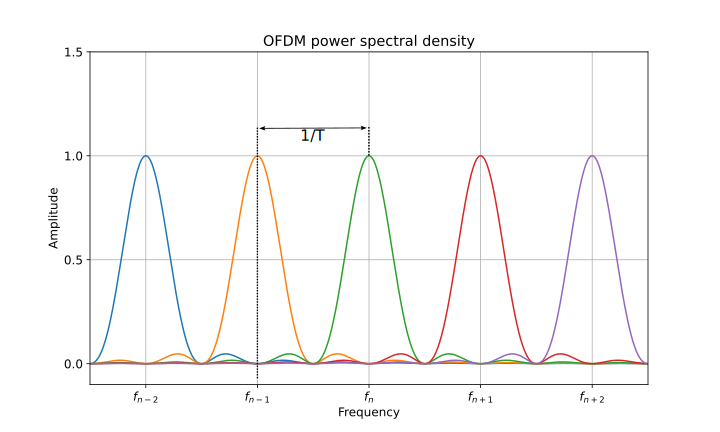
\includegraphics[width=0.7\textwidth]{Images/theoretical/ofdm/ofdm_psd_mod.png}
    \caption{Example of power spectral density of an OFDM signal with $N$ = 5.}
    \label{fig:quadtree}
\end{figure}

\subsection{Subcarriers and frequency spacing}
An OFDM system is based on the use of \textit{N} subcarriers, namely with frequencies $f_0$ to $f_{N-1}$, and $M$ time-slots that will limit the temporal length of the OFDM signal.
Each set of modulated data transmitted in a single time slot will be referred as an OFDM \textit{symbol}, while the entirety $N\times M$ symbols is referred to as an OFDM \textit{frame}.

Orthogonality of subcarriers is guaranteed by a frequency spacing $\Delta f$ of $1/T$, where $T$ is the duration of a single rectangular baseband pulse.
The time-domain signal can be expressed as

\begin{equation}
    s(t) = \sum_l\sum_{i=0}^{N-1} a_{i,l}\cdot \sqrt{\frac{1}{T}} \mathrm{rect} \left( \frac{t-T/2 - lT}{T} \right)\exp{\left(\frac{j2\pi it}{T}\right)},
\end{equation}

where $a_{i,l}$ is the complex QAM symbol modulating the \textit{i-th} subcarrier in the \textit{l-th} symbol interval.

\subsection{Implementation}
The relation between the discrete samples of OFDM in the time and frequency domain enables a beneficial implementation.
Sampling the signal at time $T/N$ we obtain a discrete version

\begin{equation}
    s_k = s(t)|_{t=k \frac{T}{N}} = \sqrt{\frac{1}{T}}\sum_{k=0}^{N-1} a_k \cdot e^{j2\pi ki/N},
\end{equation}

which is a \gls{dfs}. When \textit{N} is a power of 2, the \gls{dfs} can be implemented in an efficient way by the \gls{ifft} algorithm.
Binary data is transmitted by organizing it into $N$ parallel complex modulated symbols. These symbols are then mapped to subcarriers in the frequency domain, and the time domain signal is obtained by adding the cyclic prefix and using the \gls{ifft}. Figure \ref{fig:ofdm_transmit} shows the scheme for transmission of an \gls{ofdm} signal.

\begin{figure}[H]
	\centering
	\includegraphics[width=0.7\textwidth]{Images/theoretical/ofdm/ofdm_transmit.png}
	\caption{OFDM transmitter scheme. \alert{MIGLIORA CAPTION}}
	\label{fig:ofdm_transmit}
\end{figure}

At the receiver, the time domain signal is sampled and each complex symbol is recovered by means of the \gls{fft} algorithm, as shown in Figure \ref{fig:ofdm_receive}.

\begin{figure}[H]
	\centering
	\includegraphics[width=0.7\textwidth]{Images/theoretical/ofdm/ofdm_receive.png}
	\caption{OFDM receiver scheme. \alert{MIGLIORA CAPTION}}
	\label{fig:ofdm_receive}
\end{figure}

\subsection{Guard interval and cyclic prefix}
A frequency selective channel will apply a time-dispersion effect on the OFDM signal. This causes each symbol to "leak" into the adjacent ones, leading to \gls{isi}.
In addition to \gls{isi}, also inter-carrier interference can be observed due to the loss of orthogonality of carriers.

\begin{figure}[t]
	\centering
	
	\subfloat[Effect of time delay on transmitted OFDM symbols. At the receiver, the first symbol is delayed and leaks into the FFT block of the following symbol.\label{fig:OFDM_no_cp_isi}]{%
		\includegraphics[scale=0.18]{Images/theoretical/ofdm/no_cp_isi.png}%
	}
	\vspace{0.5cm}
	\subfloat[Effect of time delay on symbols with CP. The delayed symbol is circularly shifted in the same FFT block. Symbol and delay can be resolved.\label{fig:OFDM_cp_isi}]{%
		\includegraphics[scale=0.18]{Images/theoretical/ofdm/cp_isi.png}%
	}
	
	\caption[]{Example of the working of cyclic prefix in OFDM.}
	\label{fig:OFDM_cyclic prefix}
\end{figure}

To avoid this effect, a guard interval is added to each \gls{ofdm} symbol. Typically its duration is $T_G = T/8$ or $T_G = T/4$, and the total \gls{ofdm} symbol duration then becomes $T_s = T + T_G$.
Due to the circular property of the discrete inverse Fourier transform, extending the time duration of the \gls{ofdm} symbol by a guard time is equivalent to prepending a copy of the last $T_G/T$ fraction of the symbol, resulting in the \gls{cp}.

% TODO: insert scheme of OFDM communication

A more thorough theoretical examination of \gls{ofdm}, multicarrier communications and their applications can be found in \cite{OFDMWireless}, \cite{Proakis_2001}.


\section{Signal processing for OFDM radar}
\label{sec:OFDM_radar_theory}
        
    During the radar operation each \gls{ofdm} frame is reflected by passive targets. The received signal is a superposition of the effect of the reflection of all the targets hit by the wave front, as described by Braun in Section 3.2 of \cite{Braun2014OFDMRA}. For the sake of practicality, this brief summary will use the same terminology and notation.
    The received signal when illuminating $H$ targets in an \gls{awgn} channel is then
    
    \begin{equation}
    \label{eq:received_signal_mltiple_targets}
        r(t) = \sum_{h=0}^{H-1} b_h s(t-\tau_h)e^{j2\pi f_{D,h}t}e^{j\hat{\varphi}_h} + z(t),
    \end{equation}
    
    where $s(t)$ is influenced by the following factors:
    
    \begin{itemize}
        \item Magnitude attenuation factor $$b_h = \sqrt{\frac{c_0\sigma_{RCS,h}}{(4\pi)^3 d_h^4f_C^2}},$$
    which depends on the distance of the target $d_h$, its \gls{rcs}, the speed of light $c_0$ and the carrier frequency $f_C$.
    
        \item Time delay $\tau_h = \frac{2d_h}{c_0},$ which is the round trip time of the reflected signal.
    
        \item A Doppler shift term introduced by the relative speed of the target $f_{D,h} = \frac{2v_{rel,h}}{c_0}f_C$.
        \item A random phase rotation $\varphi_h$.
        \item \gls{awgn} $\hat{z}(t)$.
    \end{itemize}
    
    Following Braun's notation \cite{Braun2014OFDMRA}, each transmitted \gls{ofdm} frame is indicated as
    \begin{equation}
        \mathbf F_{Tx} = \begin{pmatrix}
            a_{0,0} & \cdots & a_{0,M} \\
            a_{1,0} & \cdots & a_{1,M} \\
            \vdots   & \ddots & \vdots \\
            a_{N-1, 0} & \cdots & a_{N-1, M} \\
        \end{pmatrix} \in \mathbbm{C}^{N\times M},
    \end{equation}
    
    where rows are different subcarriers, columns are different time slots and $a$ is a symbol belonging to a complex modulation.
    The received frame matrix $\mathbf F_{Rx}$ is obtained by analog/digital conversion of the signal, removal of \gls{cp} from each OFDM symbol, and computing the \gls{fft} of length $N$ for every column of the matrix, as presented in Figure~\ref{fig:ofdm_receive}.
    
    \subsection{Effect of targets on OFDM frames}
    Figure \ref{fig:sensing_operation} depicts the scheme of a radar system.
    Each target reflection will affect different elements of the frame in a different way:
    \begin{enumerate}
        \item A Doppler frequency shift $f_D$ is equivalent to modulating the elements of each row of $\mathbf F_{Tx}$ by a factor $e^{j2\pi f_D T_S l},\quad  l = 0, \cdots, M-1$.
        \item A round trip delay $\tau$ will influence each subcarrier differently, based on its frequency. The corresponding phase shift on the k-th subcarrier is \\$e^{-j2\pi (k\Delta f + f_0)\tau} \quad  k = 0, \cdots, N-1$.
    \end{enumerate}
    For the single target case, $H=1$, the received OFDM frame will become
    \begin{equation}
        (\mathbf F_{Rx})_{k,l} = b_0(\mathbf F_{Tx})_{k,l} \cdot e^{j2\pi T_S f_{D,0} l}\cdot e^{-j2\pi k \tau_0 \Delta f} \cdot e^{j\varphi_0} + (\mathbf{\Tilde{Z}})_{k,l}.
    \end{equation}
    The received frame $\mathbf{F}_{Rx}$ contains contributions from the parameters $\tau$ and $f_D$, the phase and magnitude parameters $\varphi$ and $b$, and from the transmitted frame $\mathbf F_{Tx}$.
    The latter does not contribute to the sensing purpose, and it can be removed from $\mathbf F_{Rx}$ by element-wise division.
    The \gls{csi} $\mathbf F$ is obtained as
    \begin{equation}
        (\mathbf F)_{k,l} = \frac{(\mathbf F_{Rx})_{k,l}}{(\mathbf F_{Tx})_{k,l}} = b_0 \cdot e^{j2\pi T_S f_{D,0} l}\cdot e^{-j2\pi k \tau_0 \Delta f} \cdot e^{j\varphi_0} + \frac{(\mathbf{\Tilde{Z}})_{k,l}}{(\mathbf F_{Tx})_{k,l}}\label{eq:CSI_frame}.    
    \end{equation}
    An alternative noise matrix $(\mathbf{Z})_{k,l}$ can be defined since the noise process will be white if $(\mathbf{\Tilde{Z}})$ is white after division by the transmitted frame.
    Finally, we generalize the result to H targets by reintroducing the sum from~\eqref{eq:received_signal_mltiple_targets}:
    \begin{equation}
        (\mathbf F)_{k,l} =  \sum_{h=0}^{H-1} b_h \cdot e^{j2\pi T_S f_{D,h} l}\cdot e^{-j2\pi k \tau_h \Delta f} \cdot e^{j\varphi_h} + (\mathbf{Z})_{k,l}.
    \end{equation}
    
    \begin{figure}[t]
    	\centering
    	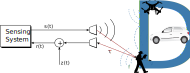
\includegraphics[width=0.9\textwidth]{Images/introduction/sensing_operation.png}
    	\caption{Schematic of a sensing (radar) system. Each target reflection affects the signal by introducing a round-trip delay $\tau$ and a Doppler shift $f_D$.}
    	\label{fig:sensing_operation}
    \end{figure}
    
    \subsection{Radar problem formulation}
    
    The estimation of the round-trip delay and of the Doppler shift for each target is equivalent to a spectral estimation problem. As Braun describes it \cite{Braun2014OFDMRA}: \textit{"Estimation of frequencies of a superposition of discretely sampled complex sinusoids, and their number"}.
    Multiple methods can be considered to solve this problem. They can be categorised as parametric, semiparametric, or nonparametric \cite{Stoica_New_Method_Parameter_Estimation}. 
    In the nonparametric class the most established method is the periodogram (also referred to as single-frequency least-squares method), which gives optimal results for sinusoids that are well resolved.
    Other established methods, which are more computationally expensive in general, are MUSIC and ESPRIT, belonging to the parametric class.
    
    \alert{This work focuses on spectral estimation based on the periodogram, which is a computationally efficient technique compared to MUSIC and ESPRIT.}
    The reduced computational complexity is crucial for the realization of a system that can process radar data in real-time without excessive overhead that may require specialized hardware.
    Although an efficient method for estimating the 2D MUSIC spectrum in 5G and 6G sensing have been proposed in \cite{Henninger_Mandelli_Arnold_EfficientMUSIC}, identifying eigenvalues corresponding to \gls{nlos} components among clutter returns from reflections can be challenging and processing time remains high due to the the large \gls{csi} and the number of targets in the scene.
    
    
    \subsection{Assumptions for OFDM radar systems}
    \label{sub:assumptions_ofdm_radar}
    The following assumptions on the \gls{isac} system simplify the design of the sensing algorithm, as described in section 3.2.1 of \cite{Braun2014OFDMRA}.
    
    \begin{enumerate}
    	\item No other distortion than \gls{awgn} is induced by the transmit and receive front-ends.
    	\item The \gls{cp} duration is larger than the round-trip propagation time for the furthermost target.
    	\item The subcarrier distance is at least one order of magnitude larger than the largest occurring Doppler shift.    	
    	\item The Doppler shift is the same on every subcarrier.
    	\item The target’s distance remains constant during the transmission of one frame.
    	
    	These assumptions are approximations of the actual conditions, as they are never exactly true for non-zero Doppler shifts. However, they are good approximations if the center frequency of the system is far greater then the total bandwidth and if the OFDM frames duration remains in the order of milliseconds.
    	Assumptions 2 and 3 ensure that the received matrix will not undergo de-orthogonalisation, which is necessary for element-wise division in Equation \eqref{eq:CSI_frame}. These conditions ensure that the \gls{ofdm} symbols are not delayed more than the \gls{cp} and are not shifted by a large Doppler shift. If these conditions are met, demodulation can occur correctly.
    \end{enumerate}
    
    \subsection{Non ambiguous range and speed}
    
        Due to the discrete nature of $\mathbf{F}$, range and speed measurements can be estimated without ambiguity if $|T_S f_D| < 1/2$ and $\tau \Delta f < 1$ are true.
        From this, the unambiguous range and speed values of the system can be derived as:
        
        \begin{itemize}
            \item Max unambiguous range
            \begin{equation}
            	d_{unamb} = \frac{c_0 \tau_{unamb}}{2} = \frac{c_0}{2\Delta f}.
            \end{equation}
            \item Max unambiguous speed
            \begin{equation}
				v_{unamb} = \frac{f_{D,unamb} c_0}{2f_C} = \frac{c_0}{2f_C T_S}.
			\end{equation}
        \end{itemize}
        
        As long as the target range and speed fall under $d < d_{unamb}$ and $|v| < v_{unamb}$ there will be no errors due to aliasing.
        
    \subsection{Range and speed resolution}
    
        Range and speed resolution depend on bandwidth and time aperture, respectively. These depend on the number of subcarriers and symbols in the \gls{ofdm} frame.
        
        \begin{itemize}
            \item Range resolution
            \begin{equation}
            	d_{res} =  \frac{c_0}{2\Delta f M}.
            \end{equation}
            \item Speed resolution
            \begin{equation}
            	v_{res} = \frac{c_0}{2 T_S f_C N}.
            \end{equation}
        \end{itemize}
        

        
\section{Periodogram-based estimation algorithms}
    
    A periodogram is defined as the estimator of the \gls{psd} of a signal.
    Considering a discrete-time signal $s(k)$ of length $N$ samples, the periodogram is defined as
    
    \begin{equation}
        \text{Per}_{s(k)}(f) = \frac{1}{N}\left| \sum_{k=0}^{N-1} s(k)e^{-j2\pi fk}\right|^2.
    \end{equation}

    The optimal way to obtain the periodogram in digital systems is by quantizing the frequency at regular intervals and using the \gls{fft} algorithm.

    \begin{align}
        \text{Per}_{s(k)}(f) &= \frac{1}{N}\left| \sum_{k=0}^{N-1} s(k)e^{-j2\pi \frac{nk}{N_{Per}}}\right|^2 \\
        &= \frac{1}{N}\left| \text{FFT}_{N_{Per}}[s(k)]\right|^2.
    \end{align}
    
    
    The transform is indicated as $\text{FFT}_{N_{per}}$ where $N_{Per} \geq N$ is the length of the \gls{fft}. When the input signal has $N < N_{Per}$, it is zero padded to the length of the \gls{fft}.
    The transform can be calculated in the most efficient way when $N_{Per}$ is a power of 2, hence it is recommended to zero-pad the input signal to the closest one.

    The input data for the periodogram is the \gls{csi} $\mathbf F$, and the periodogram is estimated in two dimensions

    \begin{equation}
    	\label{eq:periodogram_full}
    	\begin{aligned}
    		\text{Per}_{\mathbf F}(n,m) &= \frac{1}{NM} \left| \underbrace{ \sum_{k=0}^{N_{Per}-1}  \overbrace{\left(  \sum_{l=0}^{M_{Per}-1} (\mathbf F)_{k,l} e^{-j2\pi \frac{lm}{M_{Per}}} \right)}^{\text{N FFTs of length $M_{Per}$}}  e^{j2\pi\frac{kn}{N_{Per}}}}_{ \text{$M_{Per}$ iFFTs of length $N_{Per}$ }} \right| ^ 2 \\
    		&= \frac{1}{NM} \left| \text{CPer}_{\mathbf F}(n,m) \right| ^ 2.
    	\end{aligned}
    \end{equation}


    Each target captured in the CSI, \ie a sinusoid in $\mathbf F$, results in a peak in $Per_{\mathbf F}(n,m)$.
    For each target, the frequencies of its sinusoids $\hat{\Omega}_d$ (column-wise) and $\hat{\Omega}_v$ (row-wise) in $\mathbf F$ will correspond to peaks at position $(\hat{n}, \hat{m})$ in the periodogram. Inversely, if $\text{Per}_{\bm{F}}(\hat{n},\hat{m})$ is a peak value, then the corresponding oscillation frequencies in $\mathbf F$ are $\hat{\Omega}_d = 2\pi\hat{n}/N_{\text{Per}}$ column-wise and $\hat{\Omega}_v = 2\pi\hat{m}/M_{\text{Per}}$ row-wise.
    
    These frequencies are converted into distance and relative speed as

    \begin{equation}
        \hat{d} = \frac{1}{2}\hat{\tau}c_0 = \frac{\hat{\Omega}_d c_0}{2 (2\pi) \Delta f} = \frac{\hat{n}c_0}{2\Delta f N_\text{Per}}
    \end{equation}
    
    and
    \begin{equation}
    	\hat{v} = \frac{\hat{f}_D c_0 }{2 f_C} = \frac{\hat{\Omega}_v c_0}{2(2\pi)f_CT_S} =  \frac{\hat{m}c_0}{2f_cT_S M_{\text{Per}}}.,
    \end{equation}
    respectively.
    As demonstrated by Braun, computing the periodogram results in a \gls{snr} gain of a factor $NM$. The numerator in~\eqref{eq:periodogram_full} is an accumulation of all the elements in $\mathbf F$, whereas the denominator is a superposition of complex Gaussian random variables.
    
	\subsection{Window functions}
	
	Window functions are commonly applied to signals when computing the periodogram. This operation is done to tune the sidelobe level and enable precise detection of targets. 
	
	The two dimensional window matrix to be applied to the periodogram $\mathbf W \in \mathbb{R}^{N\times M}$ is multiplied element-wise with the matrix $\mathbf F$. When computing the periodogram, Equation~\eqref{eq:periodogram_full} becomes
	
	
	   \begin{align}
		\text{Per}_{\mathbf F}(n,m) &= \frac{1}{NM} \left| \underbrace{ \sum_{k=0}^{N_{Per}-1}  \overbrace{\left( \sum_{l=0}^{M_{Per}-1} (\bm{F})_{k,l} (\mathbf W)_{k,l} e^{-j2\pi \frac{lm}{M_{Per}}} \right)}^{\text{N FFTs of length $M_{Per}$}}  e^{j2\pi\frac{kn}{N_{Per}}}}_{ \text{$M_{Per}$ iFFTs of length $N_{Per}$ }} \right| ^ 2\\
		&= \frac{1}{NM} \left| \text{CPer}_{\bm{F}}(n,m) \right| ^ 2.
		\end{align}
	 
	 If no windowing is considered, then $(\mathbf W)_{k,l} = 1$ as in a simple boxcar window.
	 In the proposed \gls{ofdm} radar system, the following window types are of interest (Figure~\ref{fig:OFDMwin_functions})~\cite{Braun2014OFDMRA},~\cite{SASPWEB2011}:
	 
	 \begin{itemize}
	 	\item Rectangular (Boxcar) windows.
	 	\item Hamming windows.
	 	\item Hann windows.
	 	\item Dolph-Chebyshev windows.
	 \end{itemize}
	
	
	Since the width of the main lobe and the height of its peak is different from each window the windowing operation results in an \gls{snr} loss when computing the periodogram.
	The overall \gls{pg} can be updated as
	
	\begin{align}
		PG = 10\log_{10}(NM) + \text{SNR}_{\bm{w}_d} + \text{SNR}_{\bm{w}_v},
	\end{align}
	
	where the \gls{snr} for each direction is equal to the DC bin of the periodogram of each window normalized by the width of the rectangular window.
	
	\begin{figure}[H]
		\centering
		
		\subfloat[One-dimensional representation of the windows in time or frequency samples. Windows are normalized to unit energy.\label{fig:OFDMwin}]{%
			\includegraphics[scale=0.7]{Images/theoretical/windows/window_functs.eps}%
		}
		\vspace{0.5cm}
		\subfloat[Window functions in frequency domain, normalized to peak power of rectangular window.\label{fig:OFDMwin_freq}]{%
			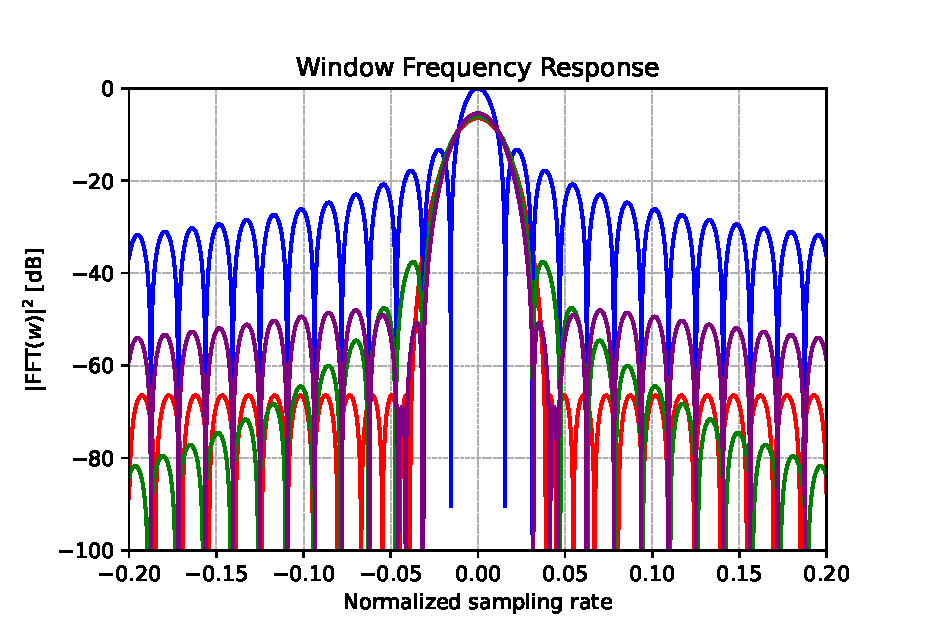
\includegraphics[scale=0.7]{Images/theoretical/windows/window_functs_freq.eps}%
		}
		
		\caption[]{Window functions available for generating the periodogram.}
		\label{fig:OFDMwin_functions}
	\end{figure}
	
	
	
	
	\subsection{Welch's method}
	
	This method, also known as \gls{wosa}, is a method for reducing the noise of the estimated spectra, by averaging independent periodograms, in exchange for a reduction in frequency resolution.
	It is based on averaging of the periodograms after the segmentation of the data into smaller segments, with some overlap if windowing is adopted \cite{Welch_period}, \cite{Spagnolini_ch14}.
	The signal is divided into $K$ data segments of $J$ samples, the periodogram is then computed separately for each segment and then averaged.
	For a one-dimensional time signal $x(t)$ \cite{SASPWEB2011}, the $k$th windowed frame is
	
	\begin{align}
		x_k(j) = w(j)x(j + kR), \; k=0,1,\ldots, K-1, j=0,1,\ldots, J-1,
	\end{align}
	
	where $R$ is the window's hop size.
	After zero padding each frame to length $J'$, where $J' > J$, the $k$th windowed and zero padded frame becomes
		\begin{align}
		x_k(j) = w(j)x'(j + kR), \; k=0,1,\ldots, K-1, j=0,1,\ldots, J'-1.
	\end{align}
	The periodogram of the \textit{k}-th block is obtained as
	
	\begin{align}
		\text{PER}_{x_k,K}(w_k) = \frac{1}{K} |\text{FFT}_{J,k}(x_k)|^2 = \frac{1}{K}\left|\sum_{j=0}^{J-1}x_k(j)e^{-j2\pi jk/J}\right|^2.
	\end{align}
	
	The Welch estimate of the \gls{psd} is then given by
	
	\begin{align}
		\hat{S}^W_x(w_k) = \frac{1}{J}\sum_{k=0}^{K-1}\text{PER}_{x_k,K}(w_k).
	\end{align}
	
	The overall data can be windowed before computing the periodogram, reducing sidelobe level in the spectral estimate, at the expense of frequency resolution. If $w(j)$ is a rectangular window, then the periodograms are formed from non-overlapping successive blocks of data (we can refer to this case as Barlett's method). For different kinds of windows the hop size $R$ should not exceed half of the frame length $J/2$. In general $R$ is chosen so that consecutive windows overlap and add to a constant.
	
	
	

\section{ISAC Proof of Concept by Nokia}
\label{sec:intro-PoCarchitecture}

The architecture considered in this work is based on \gls{fr2} 5G commercially available communication hardware.
The system consists in a mmWave \gls{gnb} \gls{ru}, extended by a dedicated \gls{ru} called \textit{Sniffer} and a server called \gls{spu}. 
The Sniffer is synchronized with the \gls{gnb} by the same synchronization source \cite{Wild_Grudnitsky_Mandelli_Henninger_Guan_Schaich_2023}. 
A schematic representation of the PoC and its building blocks is shown in Figure \ref{fig:Overview_PoC_scheme}.

As presented in Section \ref{sec:OFDM_radar_theory}, in order to apply the OFDM radar approach, one must know the TX symbols at RX and obtain the CSI by removing their influence via element-wise division \cite{Braun2014OFDMRA}. 
Using Option 7-2 of the possible 5G splits \cite{Larsen_Checko_Christiansen_2019}, it is possible to use the same type of \gls{ru} for both communication and sensing.
Option 7-2 splits the network at the \gls{phy} level, which handles the conversion of digital data to the analogue radio signal in \gls{dl}, while doing the opposite in \gls{ul}.
This split defines the \gls{fft}/\gls{ifft} performed in the \gls{ru}, while the frequency domain IQ is transported on the fronthaul.
The \gls{spu} receives the complex IQ signal,  after \gls{fft} and removal of the \gls{cp}, as input for further sensing processing on a per-radio frame basis.

The \gls{gnb} \gls{ru} lacks full-duplex capabilities, hence it operates in \gls{tdd} mode, where \gls{ul} is separated from \gls{dl} by the allocation of different time slots in the same frequency band.
The Sniffer operates always in \gls{ul} mode, receiving both the signal transmitted by \glspl{ue} and the reflected signals. 

This work considers a \gls{poc} deployment where the primary \gls{gnb} \gls{ru} and the sniffer are mounted in proximity and are co-located, allowing the system to behave as a monostatic radar. 
The scope of this work does not cover the case of bistatic radar.

\begin{figure}[t]
	\centering
	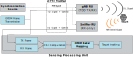
\includegraphics[width=0.9\textwidth]{Images/overview/PoC_scheme.pdf}
	\caption{Schematic of ISAC PoC with processing blocks and interfaces. }
	\label{fig:Overview_PoC_scheme}
\end{figure}

The SPU processing chain for sensing is structured as follows:

\begin{itemize}
	\item \textit{Reference and reflected signal reception}. Receive and process packets from \gls{gnb} and Sniffer. Each radio frame has dimension $N\times M$, where $N$ is the number of subcarriers and $M$ the number of \gls{ofdm} symbols.
	\item \textit{Channel computation}. Channel information is obtained by division of the received by the transmitted frames.
	\item \textit{Clutter removal}. Before every measurement, the channel of the corresponding scenario without targets is saved during a calibration step and, based on that, the clutter components are removed from the reflected signal at runtime.
	\item \textit{Periodogram computation}. The spectral response of the channel information is obtained by computing $N$ \glspl{fft} followed by $M$ \glspl{ifft} on the result. The response is then converted in a 2D range-Doppler map of the observed targets. 
	\item \textit{Peak extraction}. Identifying the peaks in the periodogram allows to retrieve the range-speed information of targets present on the scene.
	\item \textit{Target tracking}. A \gls{kf} can be used to track the detected targets. 
\end{itemize} 
A more detailed description on how the processing chain is structured,  based on \cite{Braun2014OFDMRA}, will be presented in Chapter \ref{chap:theoretical_OFDM}.


The system specifications are indicated in table \ref{table:PoCparams}.
They correspond to parameters for 5G \gls{NR} systems with the numerology $\mu=3$ specified in \cite{TS138211}. 

The system is equipped with analog beamforming and measurements can be obtained using a fixed beam for both \gls{gnb} \gls{ru} and sniffer, chosen from a beam codebook.

\begin{table}[t]
	%\caption*{\textbf{Title of Table (optional)}}
	\centering 
	\caption{List of system parameters from Nokia proof of concept installation.}
	\label{table:PoCparams}
	\begin{tabular}{|p{9em} c c |}
		\hline
		\rowcolor{bluepoli!40} % comment this line to remove the color
		\textbf{Parameter} & \textbf{Description} & \textbf{Value}  \T\B \\
		\hline \hline
		$\mu$ & 5G numerology & 3 \T\B \\
		$f_C$ & carrier frequency & 27.4 GHz \T\B \\
		$B$ & bandwidth & 200 MHz \T\B\\
		$\Delta_f$ & subcarrier spacing & 120 kHz  \T\B\\
		$T_S = 1/\Delta_f + T_{CP}$ & symbol time & 8.92 $\mu s$  \T\B\\
		$T_{CP}$ & cyclic prefix time & 0.59 $\mu s$  \T\B\\
		$N$ & number of subcarriers & 1584  \T\B\\
		$M$ & number of symbols & 1120  \B\\
		
		\hline
	\end{tabular}
	\\[10pt]
\end{table}


    
    
    

% Processing with TDD frame structure
\chapter{TDD pattern of the OFDM frame}
\label{chap:TDD pattern of the OFDM frame}


Sensing radar processing was initially carried out on a per-OFDM-frame basis. \protect\newline Every $10$ ms the system would output a received OFDM frame for radar processing, generating an update to the target state. When processing the whole frame, the number of subcarriers and symbols is rather large, resulting in good radar performance and considerable SNR gain after computing the periodogram. However, this approach suffers from the presence of unwanted spectral replicas caused by the presence of empty uplink (UL) symbols in the frame.
    
As shown in section \ref{sec:intro-PoCarchitecture}, the gNB transmits in a TDD pattern. Each pattern consists of 104 DL symbols and 36 UL symbols, repeated 8 times in each frame.

Received UL symbols do not contain any useful information for radar processing, hence they are discarded (set to zero) before computing the periodogram.

\begin{figure}[H]
    \centering
    \includegraphics[width=0.5\textwidth]{Images/TDDprocessing/CSIMatrix_DLULpattern.png}
    \caption{CSI matrix from NOKIA PoC, rows and columns correspond to OFDM subcarriers and symbols respectively}
    \label{fig:CSIMatrix_DLULpattern}
\end{figure}

\section{Ideal system performance}

Without modifying the OFDM frame, the system can carry out radar processing with the following performance:

\begin{itemize}
    \item \textbf{Unambiguous speed}
     \vspace{-\baselineskip} % Remove extra whitespace
            \begin{equation}
                v_{\text{unamb}} = \frac{c_0}{2f_C T_S} = 613.15\text{ m/s}.
            \end{equation}
           
     \item \textbf{Unambiguous range}
            \begin{equation}
                d_{\text{unamb}} = \frac{c_0}{2\Delta_f} = 1250.0\text{ m}.
            \end{equation}
     \item \textbf{Speed resolution}
            \begin{equation}
                v_{\text{res}} = \frac{c_0}{2T_Sf_CM} = 0.603 \text{ m/s}.
            \end{equation} 
     \item \textbf{Range resolution}
            \begin{equation}
                d_{\text{res}} = \frac{c_0}{2\Delta_fN} = 0.789 \text{ m}.
            \end{equation}  
\end{itemize}



\section{Effect of empty UL symbols}
    
    The removal of UL symbols acts as windowing on the received frame. This introduces additional spectral replicas in speed as shown in figure \ref{fig:SpectralReplicasDLULpattern}. Replicas seem to appear at a constant speed displacement from where actual targets lie, behaving similarly to replicas due to the radar's non-ambiguity speed.
    
    \begin{figure}[H]
        \centering
        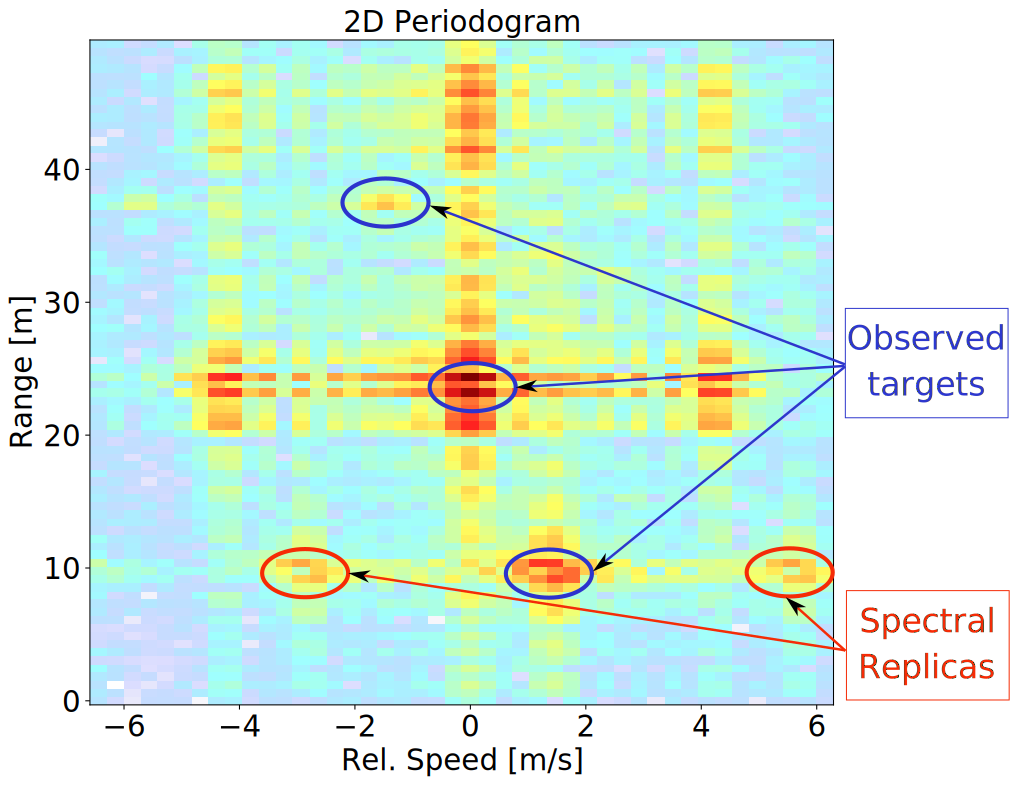
\includegraphics[width=0.55\textwidth]{Images/TDDprocessing/SpectralReplicasDLULpattern.png}
        \caption{Periodogram of a radar measurement with: static target at 23 m; moving target (range = 9.5 m, speed = 0.94 m/s); NLOS target (range = 37.2 m, speed = -1 m/s)}
        \label{fig:SpectralReplicasDLULpattern}
    \end{figure}
    
    In order to characterize the additional spectral replicas, the windowing function used to set all UL symbols to zero is analyzed. The windowing pattern can be expressed in the form
    
    \begin{align}
        &\text{rect}\left( \frac{t + \tau}{104 \cdot T_S}\right) \ast \sum_{i=0}^7 \delta\left( t - i\cdot \frac{140}{1120}\cdot T_{\text{frame}} \right),  \\
        &T_{\text{frame}} = 1120 \cdot T_S.
    \end{align}

    The windowing function, apart from a time-shift factor, is a rectangle function (Dirichlet window) convoluted with a train of Dirac deltas with spacing of 140 samples, Figure \ref{fig:TDDproc_rectfunct}. Its transform in frequency, Figure \ref{fig:TDDproc_rectfunct_transform}, is a cardinal sine function multiplied by a train of Dirac deltas.

    The transform is then convoluted with the signal in the frequency domain. The impulses adjacent to the one at zero-frequency in figure \ref{fig:TDDproc_rectfunct_transform} appear as replicas in the periodogram. These peaks have enough power to be detected as actual targets, limiting the system's performance by reducing the effective unambiguous speed or by masking actual targets that would be detected near the replica. 

\begin{figure}[H]
    \centering
    
    \subfloat[TDD windowing function\label{fig:TDDproc_rectfunct}]{%
        \includegraphics[scale=0.5]{Images/TDDprocessing/rectFunct.eps}%
    }\hfill
    \subfloat[Transform of the windowing function, FFT over 2048 points, absolute value\label{fig:TDDproc_rectfunct_transform}]{%
        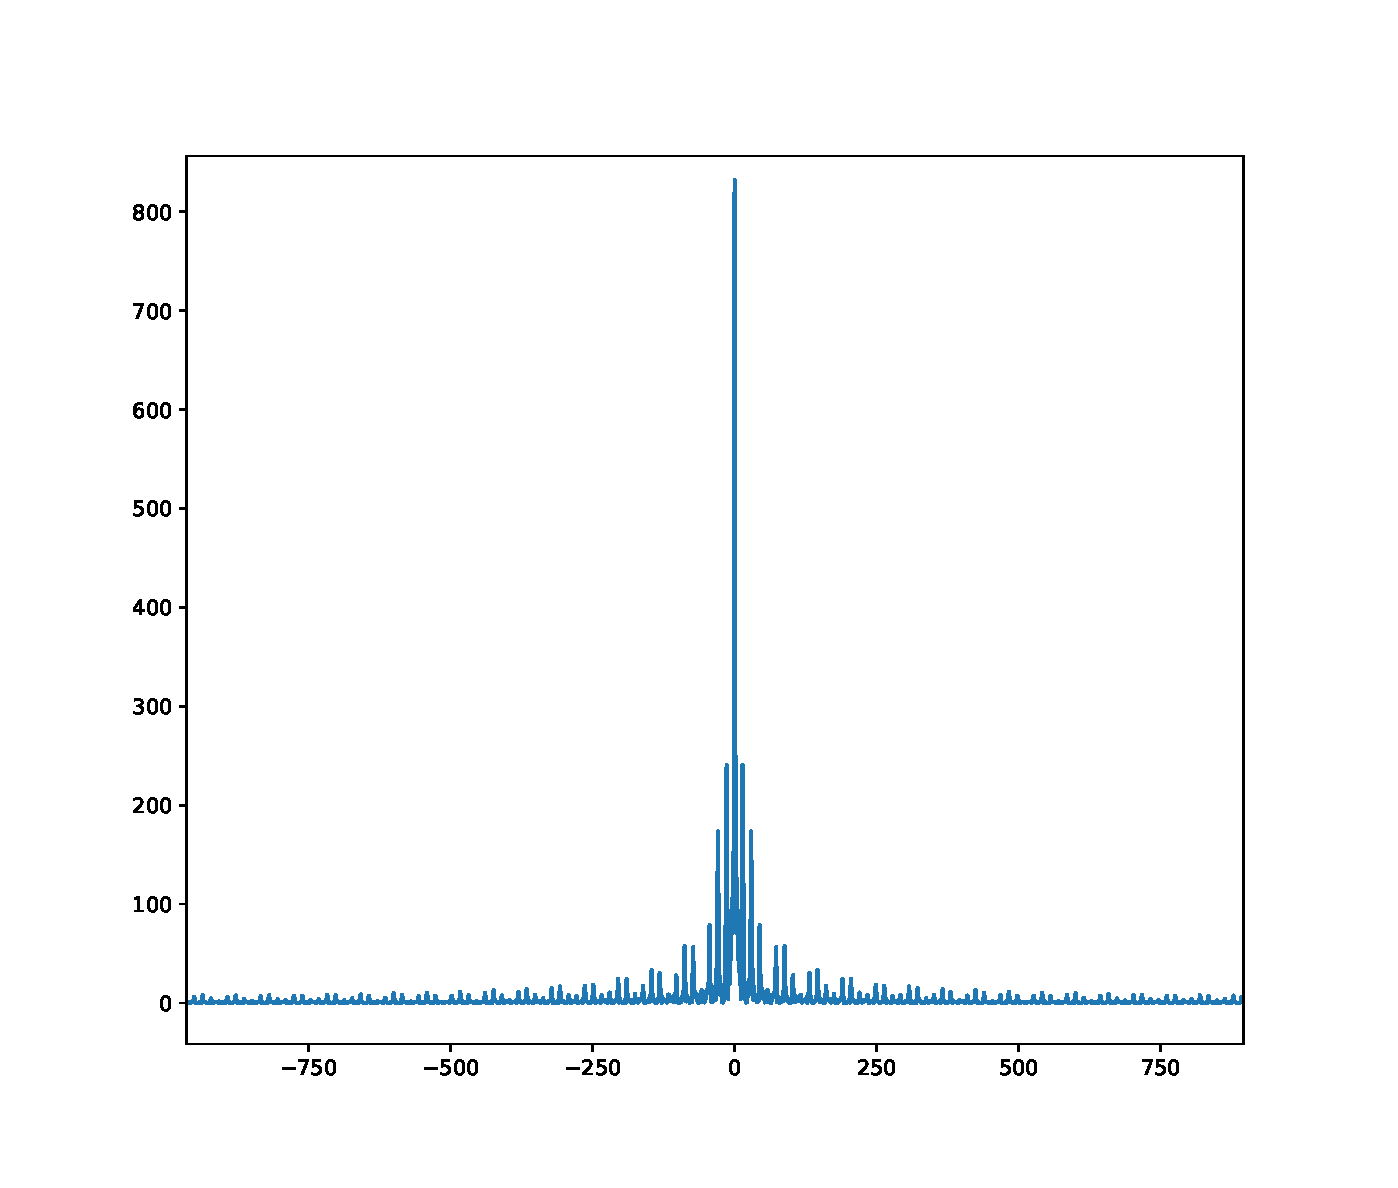
\includegraphics[scale=0.335]{Images/TDDprocessing/transform_of_rectFunct1.eps}%
    }
    
    \caption[]{}
    \label{fig:TDDwindowingfunct}
\end{figure}

\section{Frame sampling strategies}

    \begin{figure}[H]
        \centering
        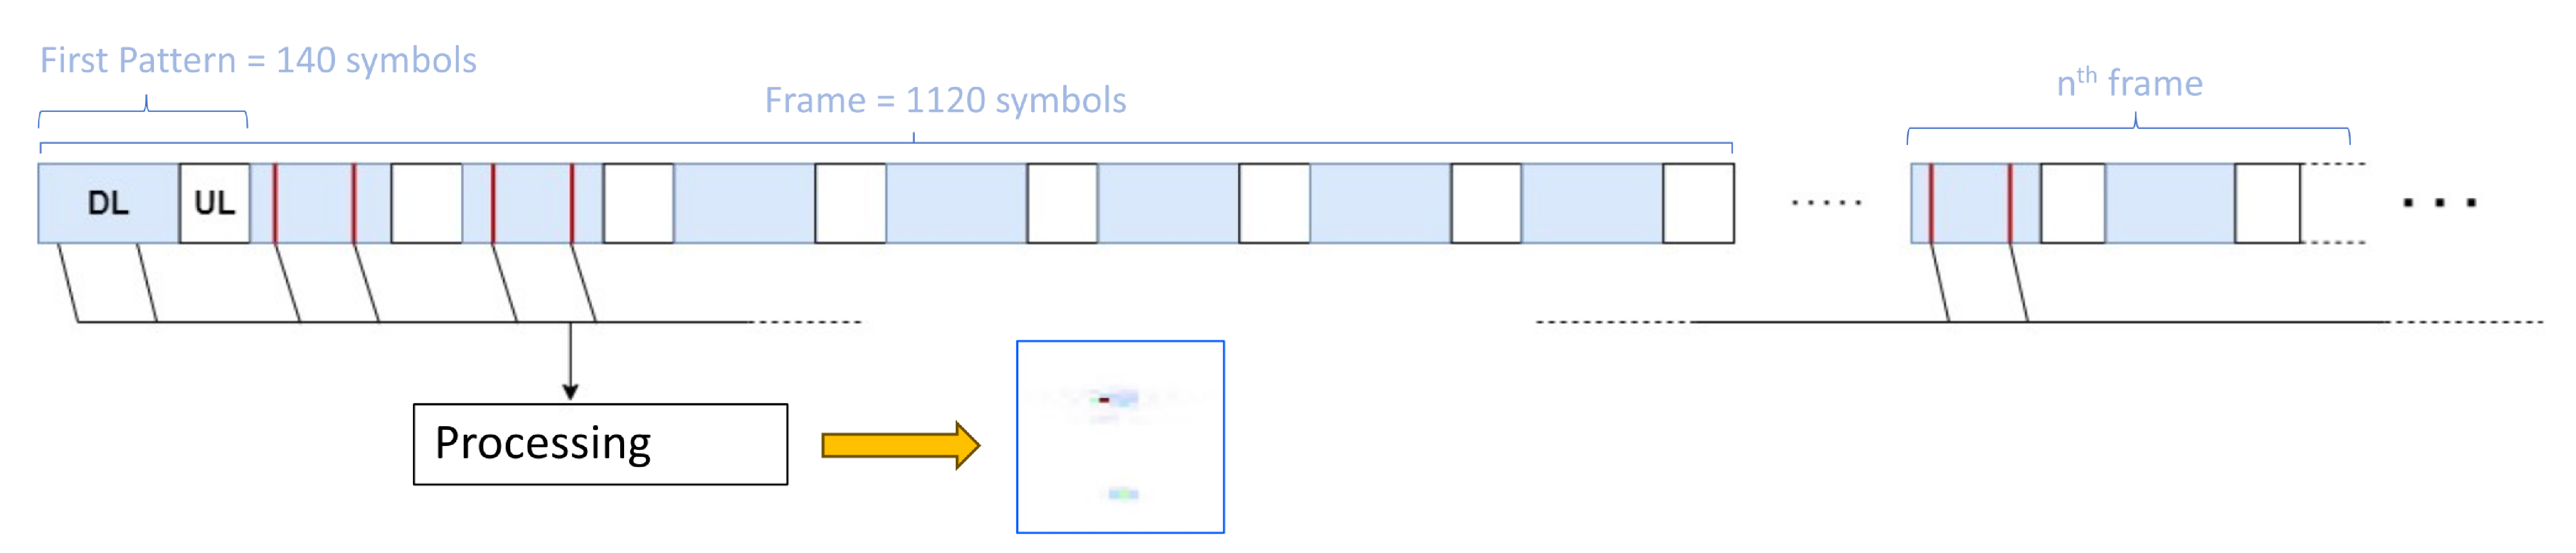
\includegraphics[width=1\textwidth]{Images/TDDprocessing/TDDstrategies.eps}
        \caption{Decimation and combining of different consecutive frames}
        \label{fig:TDDstrategies}
    \end{figure}

    \paragraph{Single DL pattern:}
    in order to avoid processing blank UL symbols, the most straightforward approach would be processing only the first 104 DL symbols. The replicas would be avoided, but the time aperture of the measure would be reduced by a factor 8, decreasing the speed resolution from $0.603$ m/s to $\approx 5.88$ m/s, unusable for most of the sensing use cases.
    
    \paragraph{Decimation at constant interval:}
     a possible strategy is re-sampling the OFDM frame in time at a fixed pace, avoiding blank symbols. Replicas are not detected, but the lower number of processed symbols translates into a considerable loss of SNR in the periodogram. This affects NLOS sensing in particular, since targets observed from a reflection present a considerably lower peak power compared with the LOS components.

     Reducing the number of available symbols with a fixed time-aperture translates in lower granularity of measurements and in a decrease in unambiguous speed. \protect\newline In the case of Figure \ref{fig:TDDperiodogram1FYesDec}, processing one symbol every 47, the obtained unambiguous speed is $13.05$ m/s. \protect\newline Speed resolution remains unchanged.
    
     \paragraph{Decimation and multi-frame processing:}
     combining consecutive frames, it is possible to process an higher number of symbols, re-gaining a part of the SNR thanks to processing gain, all without observing replicas. The time aperture of the measurement is also increased, translating into a better speed resolution.

     This approach introduces a trade-off between SNR (processing gain) and update rate. Increasing the time-aperture, some range migration effect can be observed, especially for fast moving targets. In the context of NLOS sensing, the impact of range migration on system performance is relatively minor compared to the benefits of increased speed resolution and higher signal-to-noise ratio, since the primary goal is not providing precise tracking or positioning data.


    In Figures \ref{fig:TDDperiodogram1FNoDec}-\ref{fig:TDDperiodogram10frames} it is possible to observe the effects of the various strategies when applied to a OFDM radar measurement where both the NLOS and LOS components are present for a single target.


% 2x2 figure scheme
    \begin{figure}[H]
        \centering
        
        \subfloat[Single processed frame, no decimation, SNR = 60.91 dB, \protect\newline $v_{\text{res}} = 0.603$ m/s, $ v_{\text{unamb}} = 613,15$ m/s
\label{fig:TDDperiodogram1FNoDec}]{
            \includegraphics[width=0.4\textwidth]{Images/TDDprocessing/periodogram1FNoDec.png}
        }
        \hfill
        \subfloat[Single processed frame, decimated, \protect\newline SNR = 45.16 dB, \protect\newline $v_{\text{res}} = 0.603$ m/s, $ v_{\text{unamb}} = 13.05$ m/s\label{fig:TDDperiodogram1FYesDec}]{
            \includegraphics[width=0.4\textwidth]{Images/TDDprocessing/periodogram1FYesDec.png}
        }
        
        \vspace{0.5cm}
        
        \subfloat[6 processed frames, decimated, combined, SNR = 52.35 dB, \protect\newline $v_{\text{res}} = 0.091$ m/s, $ v_{\text{unamb}} = 8.76$ m/s\label{fig:TDDperiodogram6frames}]{
            \includegraphics[width=0.4\textwidth]{Images/TDDprocessing/periodogram6frames.png}
        }
        \hfill
        \subfloat[10 processed frames, decimated, combined, SNR = 54.66 dB, \protect\newline $v_{\text{res}} = 0.054$ m/s, $ v_{\text{unamb}} = 8.76$ m/s\label{fig:TDDperiodogram10frames}]{
            \includegraphics[width=0.4\textwidth]{Images/TDDprocessing/periodogram10frames.png}
        }
        
        \caption{Examples of possible decimation and combining approaches in periodogram processing}
        \label{fig:allperiodogram-decimation}
    \end{figure}


    
\begin{table}[H]
    %\caption*{\textbf{Title of Table (optional)}}
    \centering 
    \begin{tabular}{|p{9em} c c c |}
    \hline
    \rowcolor{bluepoli!40} % comment this line to remove the color
     \textbf{Strategy} & \textbf{SNR [dB]} & \textbf{N} & \textbf{Time aperture [ms]} \T\B \\
    \hline \hline
    $\textbf{Standard frame}$ & 60.91 & 1120 & 10 \T\B \\
    $\textbf{Decimated frame}$ & 45.16 & 24 & 10 \T\B\\
    $\textbf{6 frames}$ & 52.35 & 96 & 60  \T\B\\
    $\textbf{10 frames}$ & 54.66 & 160 & 100  \T\B\\

    \hline
    \end{tabular}
    \\[10pt]
    \caption{Comparison between SNR levels for different frame processing strategies}
    \label{table:TDDstratcomparison}
\end{table}



% Radar detection and thresholding techniques
% !TeX spellcheck = <none>
%\chapter{Radar frame processing}
%\label{chap:radar_detection}

	\section{Radar search and detection}
	\label{sec:radar_search_detection}
		Detection is commonly defined as the process of analysing the radar data and determining whether it consists of noise only, or noise plus echoes coming from a target of interest~\cite{Richards_Scheer_Holm_2010}. 
		For this purpose the literature designed statistical tests aimed at deciding whether a data point consists of noise only, or noise plus echoes coming from a target of interest.
		
		Users of radar systems are typically concerned with determining (or defining) the probability of detecting a target $P_\text{D}$ and the probability of false alarm $P_\text{{FA}}$.  By using the knowledge of the desired $P_\text{{FA}}$, noise statistics, and detector design, it is possible to decide the appropriate threshold to be used at the detector's output.
		
		In this work different approaches are considered and their respective advantages and drawbacks analysed. 



		\subsection{Constant False Alarm Rate}
	
				Standard radar detection assumes the level of noise and interference to be known and constant. In this conditions it is possible to precisely determine the correct threshold for achieving the desired $	p_\text{FA}$. In real scenarios interference levels may be highly variable throughout an acquisition, making the use of a dynamic threshold necessary. Constant false alarm rate (CFAR) is an adapting threshold technique aiming at providing predictable behaviour of detection and false alarm rates in real scenarios \cite{Richards_2014}.
				
				%TODO generate image showing fixed vs adaptive threshold
				
				In OFDM radar, a \textit{false alarm} occurs when the target detector determines the presence of a target at a range and relative speed that does not contribute to the received matrix $\mathbf F_{Rx}$ \cite{Braun2014OFDMRA}. 
				Consequently, the probability of false alarm is the probability of observing a positive detection when the received frame consists only of noise $(\mathbf F_{Rx} = \mathbf Z)$. 
				This definition considers processing on a per-frame basis and can also be applied to the multi-frame processing strategies presented in Section \ref{sec:frame_sampling_strategies}. 
				
				The presence of clutter is not yet taken into account as the threshold is estimated by determining an estimator for the noise power of the processed data. 
				Furthermore, clutter can be defined as reflections generated by objects in the environment, that are not of interest for the sensing task. 
				This means that detections due to objects considered as clutter are expected and can be mitigated by various clutter removal techniques.
				
				In order to discriminate noise from signal power, the periodogram is subjected to an hypothesis test with an appropriate threshold $\eta$
				\begin{align}
					\text{Per}_{\mathbf F}(n,m) \quad\mathop{\gtrless}_{H_1}^{H_0}  \quad \eta,
				\end{align}
				where $H_0$ is the null hypothesis, target not present, and $H_1$ is the hypothesis where the reflection from a target contributes to the received power in the bin under test.\\
				The probability that any bin of the periodogram exceeds the threshold when only noise power $Z$ is present is
				\begin{align}
					p_{\text{FA},bin} = \text{Per}(Z > \eta) = \int_\eta^{\infty} f_z(z|H_0)dz = 1 - F_z(\eta | H_0) = e^{-\dfrac{\eta}{\sigma_n^2}},
				\end{align}
				 
				where $f_z(z|H_0)$ and $F_z(\eta | H_0)$ are the \gls{pdf} and \gls{cdf} of the random variable $Z$. 
				The observed noise contribution is given by the magnitude squared of the \gls{awgn} with power $\sigma_n^2$.
				Given an exponentially distributed interference, the probability of false alarm is defined as
				\begin{align}
					p_\text{FA} = \exp \left( -\frac{\eta}{\sigma_n^2}\right),
				\end{align}
			where for a fixed threshold an increase in the interference power causes an increase in $p_\text{FA}$~\cite{Richards_Scheer_Holm_2010}.
				The threshold for a given false alarm rate per bin is obtained as
				\begin{align}
					\eta = -\sigma_n^2 \ln(p_{\text{FA},bin}) .
					\label{eq:CFAR_threshold_false_alarm_1}
				\end{align} 
				For the full (non zero padded) periodogram the false alarm probability is
				\begin{align}
					p_\text{FA} = 1 - (1 - p_{\text{FA},bin})^{NM}.
				\end{align}
				Solving this for $p_{\text{FA},bin}$ in \eqref{eq:CFAR_threshold_false_alarm_1}, we obtain the value of the threshold as 
				\begin{align}
					\eta = \sigma_N^2 \ln{(1 - (1 - p_{\text{FA},bin})^{\frac{1}{NM}})}.
				\end{align}
				Zero-padding the periodogram does not add information useful for the target estimation problem, but it only reduces quantization noise. The contribution of a single bin is spread out between multiple contiguous bins when zero-padding.
				
				Optimality for this detection method and a more thorough theoretical analysis can be found in Chapter 15 of \cite{Richards_Scheer_Holm_2010}.

				\subsubsection{Estimation of noise power}
	
					Noise power is estimated from the periodogram by averaging over bins where the target is not expected.
					From Assumption 3 from Section \ref{sub:assumptions_ofdm_radar}, the maximum target delay and consequently, the maximum range bin in which we can observe a target depends on the guard interval defined by the \gls{cp}. They are calculated as 
					\begin{align}
						\tau_{\text{max}} =& \frac{N_{\text{max}}}{N_{\text{Per}}}\cdot T = T_\text{CP} ,\\
						N_{\text{max}} =& \frac{T_\text{CP}}{T}\cdot N_{\text{Per}}.
					\end{align} 
					
					The maximum likelihood estimate for the noise power is found by averaging over one or more rows beyond $N_{\text{max}}$
			
					\begin{align}
					\label{align: threshold_noise_power}
						\hat{\sigma_n}^2 = \frac{1}{M_{\text{Per}}K} \sum_{k=1}^K \sum_{m=1}^{M_{\text{Per}}} \text{Per}_{\bm{F}}(N_{\text{max}}+k, m).
					\end{align}
			
			It was observed that, when using \gls{cfar}, estimating a fixed threshold across the periodogram based only on the level of the noise floor leads to  numerous above-threshold cells due to the sidelobes of the target returns, as shown in Figure \ref{fig:RadThesh_CFAR_abv_thresh_doubl}.
			
				\begin{figure}[t]
				\centering
				
				\subfloat[Above-threshold bins, threshold estimated using CFAR.\label{fig:RadThesh_CFAR_abv_thresh}]{%
					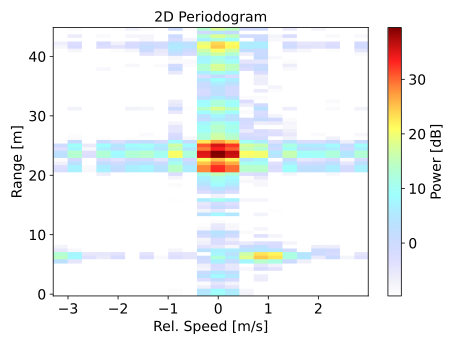
\includegraphics[scale=0.45]{Images/radar_detect_threshold/cfar_abv_thresh.png}%
				}\hfill
				\subfloat[Reference periodogram. \label{fig:RadThesh_CFAR_abv_thresh_PER}]{%
					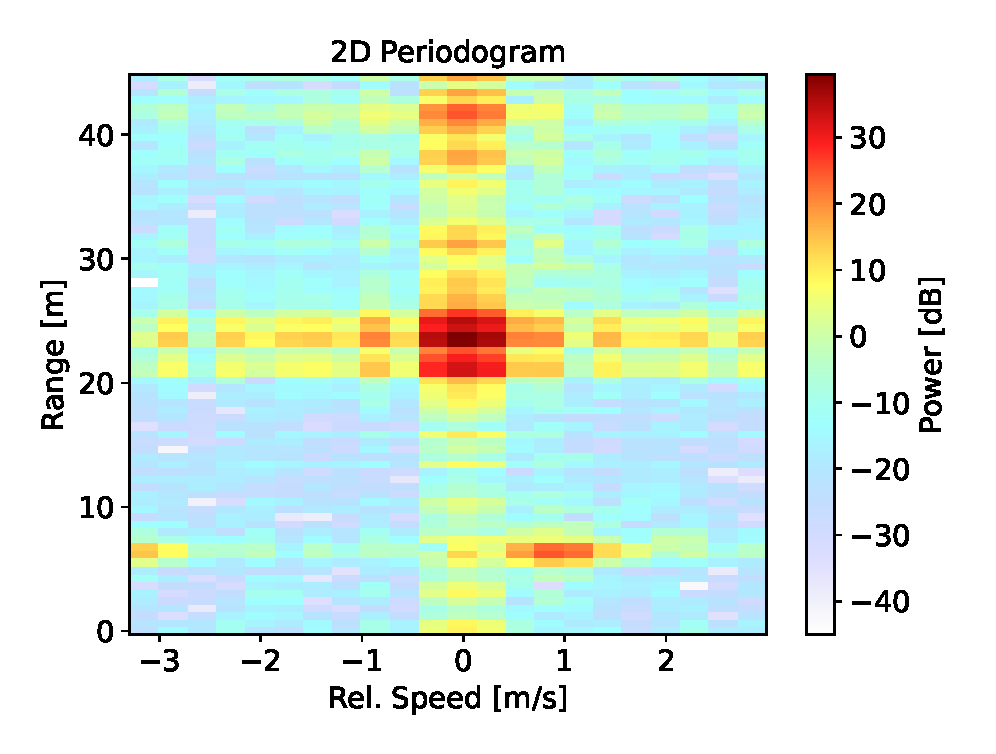
\includegraphics[scale=0.45]{Images/radar_detect_threshold/cfar_abv_thresh_PER.eps}%
				}
				
				\caption[]{Example of \gls{cfar} thresholding. It can be observed that the largest target positioned at 23 m (a wall) presents strong sidelobes that are detected as target returns.}
				\label{fig:RadThesh_CFAR_abv_thresh_doubl}
			\end{figure}
			
			
			One common method for significantly reducing false alarms after the detection process is using a confirmation system that requires each target to be detected twice: once in the initial search and in a subsequent confirmation process.
			Nonetheless, there is still the possibility that a noise spike will remain in the confirmation measure and the target will not. In addition, this approach can suffer from peaks generated by clutter or spectral artefacts that may persist over time.

		\subsection{Cell-averaging CFAR}
		\label{sec:cell averaging CFAR}

The generic CFAR detector described in the previous section defines a threshold, based on noise power, to be applied to the whole periodogram. More advanced algorithms for CFAR detection belong to the family of \gls{cacfar} \cite{Richards_2014}.

In a noisy environment, very weak echo signals may be lost in the case of a fixed threshold across the periodogram. \gls{cacfar} estimates the threshold level for each cell of the 2D periodogram based on the statistics of neighbouring cells belonging inside a set reference window. In this way noise levels are estimated for smaller sections of the periodogram, adapting to the local level of the interference and defining a variable threshold across the periodogram.
The \gls{cfar} window resides inside the data window and is composed of leading and lagging reference windows, guard cells and \gls{cut}. Guard cells are discarded for noise computation since they may contain returns associated with the target in the \gls{cut}.

In the \gls{ofdm} radar problem a two-dimensional range-Doppler \gls{cfar} window is considered, where the \gls{cut} is located at the center.

\begin{figure}[H]
	\centering
	\includegraphics[width=0.9\textwidth]{Images/radar_detect_threshold/cacfar_pipeline.png}
	\caption{CA-CFAR detection processor, guard cells are shown in red, while reference cells are green highlighted.}
	\label{fig:cacfar_pipeline}
\end{figure}


% TODO: insert CACFAR scheme from presentation (add guard cells)
% TODO: insert sliding windows

The \gls{cacfar} threshold is defined by the product of the noise power estimate and a \gls{cfar} constant

\begin{align}
	\eta_{\text{CA-CFAR},CUT} = \alpha_{\text{CA}} \hat{\sigma_n}^2.
\end{align}

The \gls{cfar} constant $\alpha_{\text{CA}}$ is a function of the probability of false alarm $p_{\text{FA}}$ and of the number of contribution cells $N$ and is derived as in Chapter 16 of \cite{Richards_Scheer_Holm_2010}. The estimated noise power is calculated as in \eqref{align: threshold_noise_power} by averaging over the contributing cells as:

\begin{equation}
	\alpha_{\text{CA}} = N[p_{\text{FA}}^{-1/N} - 1] \quad \text{and} \quad \hat{\sigma_n}^2 = \frac{1}{N}\sum_{n=1}^N z_n.
\end{equation}

The number of operations can be reduced by simplifying the normalization by $\frac{1}{N}$ by defining a noise statistics $\hat{g}_{\text{CA}}' = \sum_{n=1}^N z_n$ and by incorporating it in the CFAR constant $\alpha_{\text{CA}}' = p_{\text{FA}}^{-1/N} - 1$.

Computationally \gls{cacfar} is more demanding than other thresholding techniques, as in its fastest implementation it still requires a 2D convolution to be applied to the periodogram before computing the threshold at each bin.

\subsubsection{Performance of CA-CFAR}

The general assumption that each radar return occupies one single bin in the range-Doppler plane is not valid for \gls{ofdm} radar systems, as the \gls{psf} is influenced by a number of factors.
Zero padding and windowing in the periodogram define the width of the main lobe of the sinusoids in the 2D plane, while a large time aperture of the acquisition generally leads to a larger return due to high speed resolution and range-Doppler spreading.
Furthermore, spread targets generate bigger responses than a point scatterer, impacting neighbouring periodogram bins.

In a heterogeneous radar frame, multiple targets and changes in the interference power degrade \gls{cfar} performance. If target returns are present in the reference window, they will bias the threshold and lead to a missed detection. This phenomenon is called \textit{target masking}. An example of target masking in 1D CA-CFAR is shown in Figure~\ref{fig:target_masking_richards}~\cite{Richards_Scheer_Holm_2010}.
Another source of performance degradation is the presence of clutter, where \textit{clutter boundaries} are areas in which there is a sudden change in the statistics of the interfering power, which leads to higher threshold and missed detection.
\begin{figure}[b!]
	\centering
	\includegraphics[width=0.75\textwidth]{Images/radar_detect_threshold/target_masking_richards.png}
	\caption{\small Example of mutual target masking in CA-CFAR from \cite{Richards_Scheer_Holm_2010}. Dashed line indicates the ideal Neyman-Pearson threshold.}
	\label{fig:target_masking_richards}
\end{figure}
Performance is also strongly influenced by the design of the reference window. The window should be designed to be as small as possible, in order to reduce the computational load due to the convolution operation and not to include interfering statistics far away from the \gls{cut}. The guard interval should be sized according to the point spread function of the target return. An extended target could be counted in the reference window and lead to \textit{self masking}.
\begin{figure}[t]
	\centering
	
	\subfloat[Above-threshold bins using CA-CFAR.\label{fig:RadThesh_CA_CFAR_missed_detect}]{%
		\includegraphics[scale=0.45]{Images/radar_detect_threshold/ca_cfar_no_nlos_1.png}%
	}\hfill
	\subfloat[Reference periodogram. LOS target at 6 m and corresponding NLOS path return at 40 m, -1,5 m/s.\label{fig:RadThesh_CA_CFAR_missed_detect_PER}]{%
		\includegraphics[scale=0.45]{Images/radar_detect_threshold/ca_cfar_no_nlos_PER_1.png}%
	}
	
	\caption[]{\small Clutter-like return observed in NLOS (top-left area denoted by the blue box): CA-CFAR uses part of the point cloud to estimate noise levels and the target is not detected due to target masking.}
	\label{fig:RadThesh_CA_CFAR_missed_detect_doubl}
\end{figure}

\subsubsection{Robust CA-CFAR}
Especially in a \gls{nlos} sensing scenario, \gls{cacfar} suffers from these drawbacks due to the lower \gls{snr} of target returns caused by multiple reflections and the presence of strong static clutter components.
Additionally, target returns can occupy multiple bins in the periodogram, leading to self masking. 
As a result, they do not appear as distinct peaks, but rather are spread across neighbouring bins, which raises the \gls{cacfar} threshold and leads to missed detections, as shown in Figure \ref{fig:RadThesh_CA_CFAR_missed_detect_doubl}.
More complex \gls{cacfar} algorithms may provide better results under certain heterogeneous conditions, but at the expense of increased computational complexity, higher cost, or lower performance under non-ideal conditions.

Some of the more common variants of the algorithm are the greatest-of CA-CFAR (GOCA-CFAR) and the censored statistics CA-CFAR (CSCA-CFAR), which are designed to suppress clutter-edge false alarms and mutual target masking, respectively.
\paragraph{Greatest-of CA-CFAR:}
The interference power is calculated in the lagging and leading reference windows separately and the largest of the two is selected as the reference statistics. In the \gls{ofdm} radar signal the leading/lagging definition can be applied only in the Doppler dimension, since interference statistics is assumed homogeneous in range.
GOCA-CFAR can, in general, avoid false alarm caused by clutter returns and clutter-edge conditions. However, in NLOS sensing, where the power of the target returns is comparable to the one of spectral artifacts and clutter sidelobes, GOCA-CFAR increases the possibility of masking, especially for slow-moving targets.
\paragraph{Censored-statistics CA-CFAR:}
This algorithm considers the largest $L_c$ samples to be containing returns from interfering targets, and therefore does not consider them when computing the interference statistics. CSCA-CFAR is in general assumed to be capable of removing up to $L_c$ interfering targets.
This algorithm can be also generalised by censoring an arbitary number of samples in order to be adapted to different environments. 
The main limitation posed by this algorithm is the increased computational cost due to the necessary ordering of the interference samples.


\subsection{Range-adjusted exponential threshold}

	
	In \cite{Wagner_Feger_Stelzer_2017}, a different approach to thresholding was proposed for detecting large point clouds of radar returns in the 2D range-Doppler plane. Similar to the \gls{ofdm} radar case in this work, due to the relatively high speed resolution, returns occupy multiple cells in the periodogram and are not correctly detected by \gls{cacfar}.
	
	The idea is to adjust the threshold level accounting for the propagation loss of the target reflection, which is proportional to the square of the distance from the sensing hardware. 
	This solution was implemented combining the \gls{cfar} threshold, set as a lower bound, and the range-dependent exponential adjustement.
	The threshold for a range-bin corresponding to returns at range $d$ is
	\begin{align}
		\eta_{\text{exp}} = \eta_{\text{CFAR}} + \frac{\alpha}{d^2},
	\end{align} 
	where $\alpha$ is an adjustment factor for the exponential term. For this particular implementation it was defined as the square root of the maximum return in the periodogram
	\begin{align}
		\alpha = \sqrt{\max{ \left\{\text{Per}_{\mathbf F}(n,m)\right\} }}.
	\end{align}
	
	Unlike \gls{cacfar} where, in general, local peaks are detected, this approach will select large point clouds whithin the periodogram, as shown in Figure \ref{fig:RadThesh_exp_thresh}.
	Targets can then be detected by searching for local peaks in the areas above threshold. A more refined result can be obtained by applying clustering algorithms, such as DBSCAN.
	
		\begin{figure}[H]
		\centering
		
		\subfloat[Periodogram with target at 9 m, moving at 1 m/s. Sidelobes from the target are present.\label{fig:RadThesh_exp_thresh_baseline}]{%
			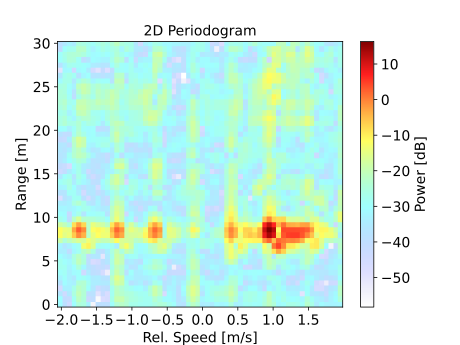
\includegraphics[scale=0.45]{Images/radar_detect_threshold/exp_thresh/per_NO_thresh.png}%
		}\hfill
		\subfloat[Above-threshold periodogram, after applying exponential threshold.\label{fig:RadThesh_exp_thresh_above}]{%
			\includegraphics[scale=0.45]{Images/radar_detect_threshold/exp_thresh/per_exp_thresh.png}%
		}
		
		\caption[]{Example of detection using the proposed range-adjusted threshold.}
		\label{fig:RadThesh_exp_thresh}
	\end{figure}
	

	\begin{figure}[!t]
	\centering
	
	\subfloat[\footnotesize no clutter removal, static metal target at range of ca. 10 m. Clutter at ca. 23 m.\label{fig:Rad_crap_ecac_base_static}]{%
		\includegraphics[scale=0.4]{Images/radar_detect_threshold/clutter/crap_ecac_static/clutter_baseline1.png}%
	}\hfill
	\subfloat[\footnotesize clutter removal with \newline ECA-C.\label{fig:Rad_crap_ecac_ECAC_static}]{%
		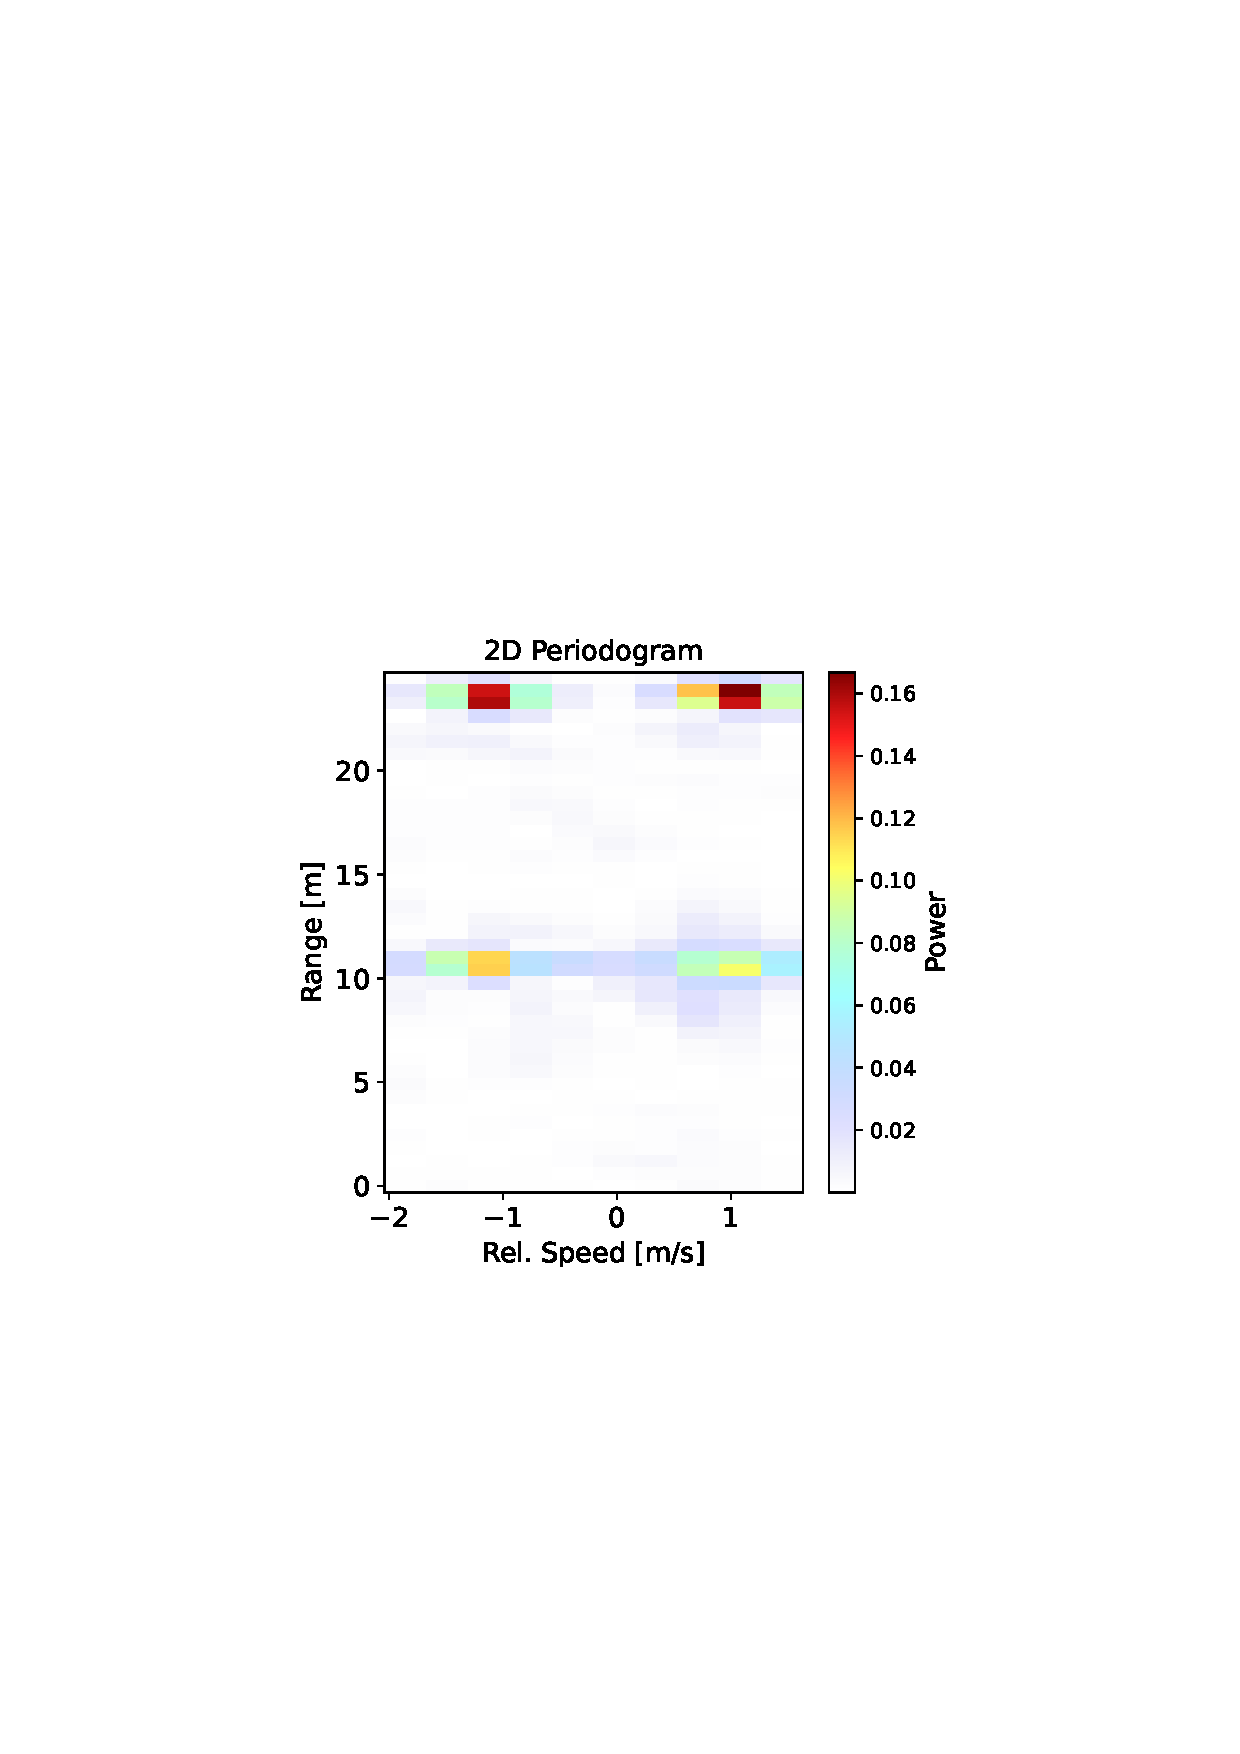
\includegraphics[scale=0.4]{Images/radar_detect_threshold/clutter/crap_ecac_static/clutter_ecac1.png}%
	}\hfill
	\subfloat[\footnotesize clutter removal using CRAP.\label{fig:Rad_crap_ecac_CRAP_static}]{
		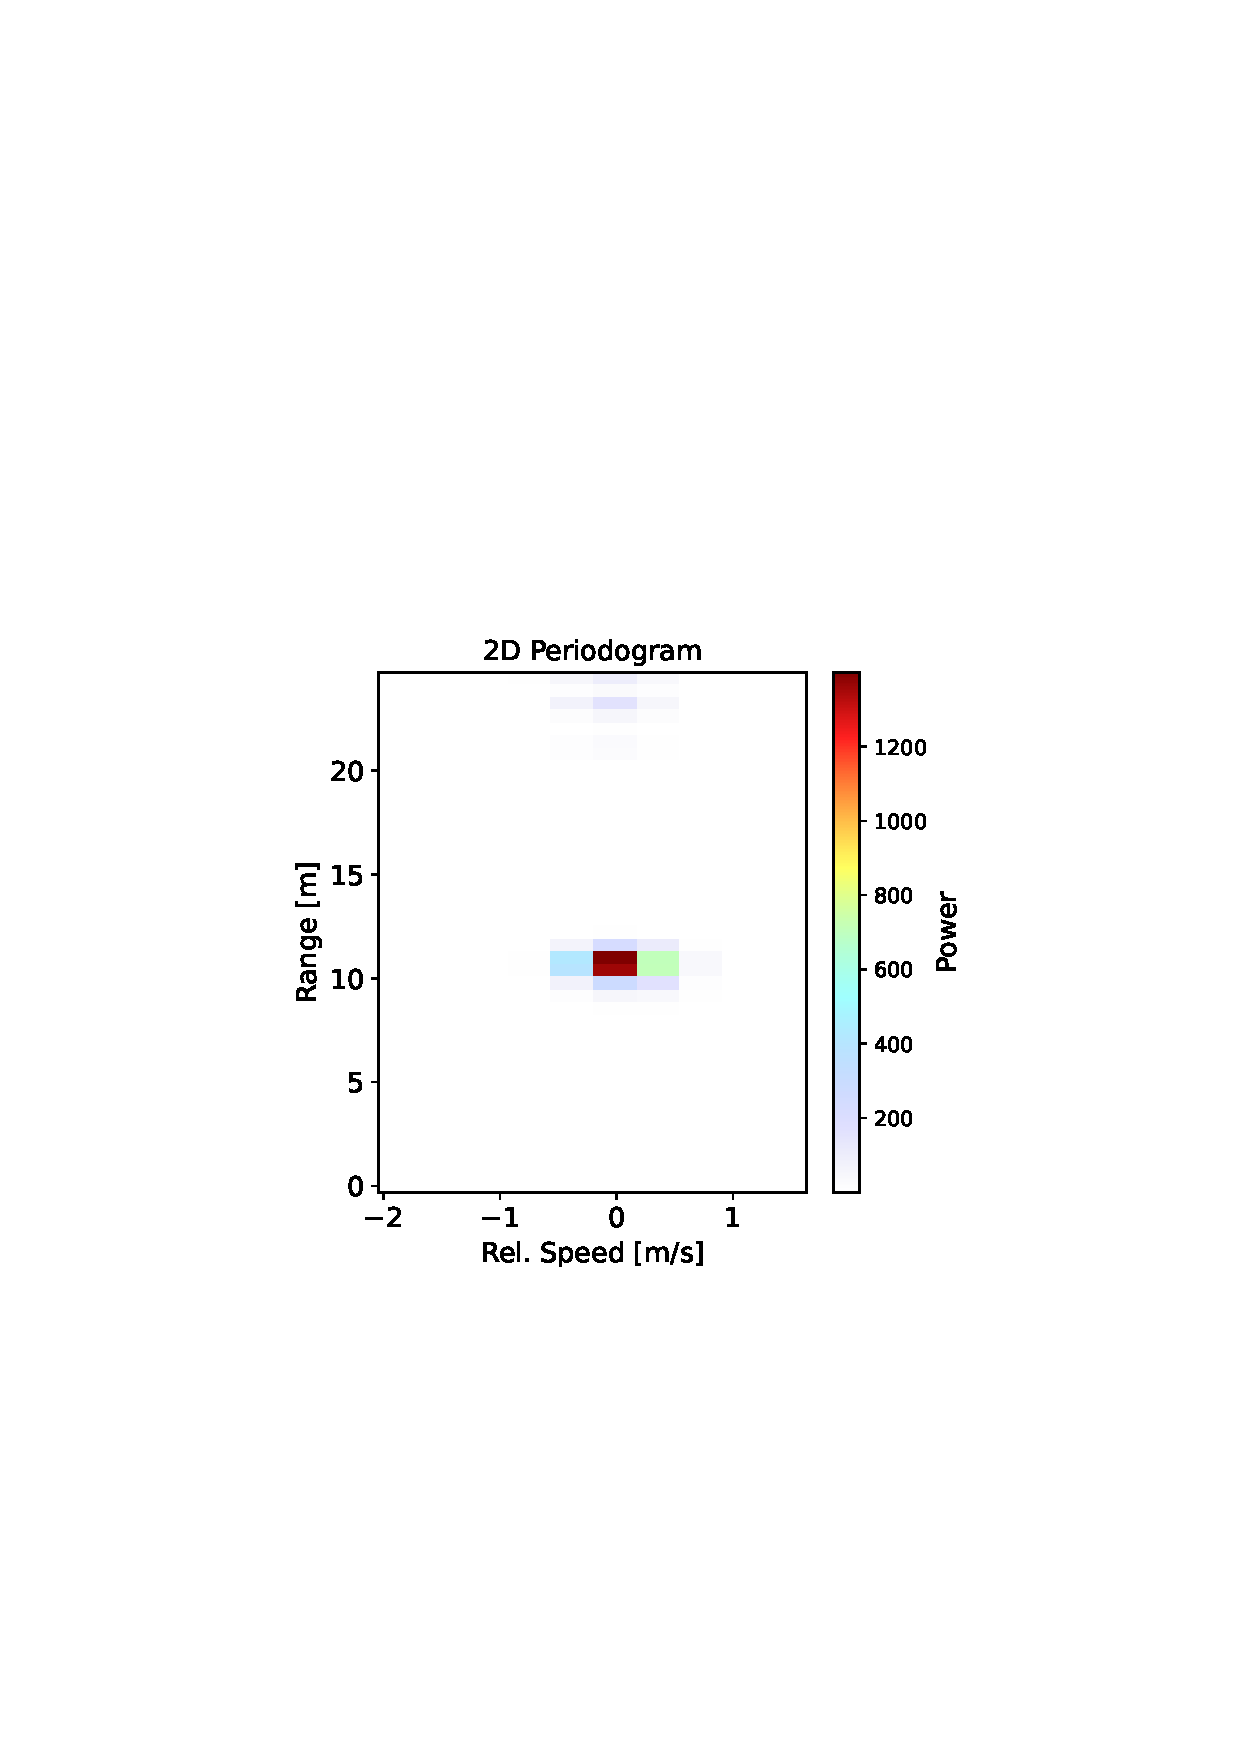
\includegraphics[scale=0.4]{Images/radar_detect_threshold/clutter/crap_ecac_static/clutter_crap1.png}
	}\newline
	
	\subfloat[\footnotesize no clutter removal, metal target at range of ca. 10 m moving at ca. 1 m/s.\newline Static clutter at ca. 23 m.\label{fig:Rad_crap_ecac_base_mov}]{%
		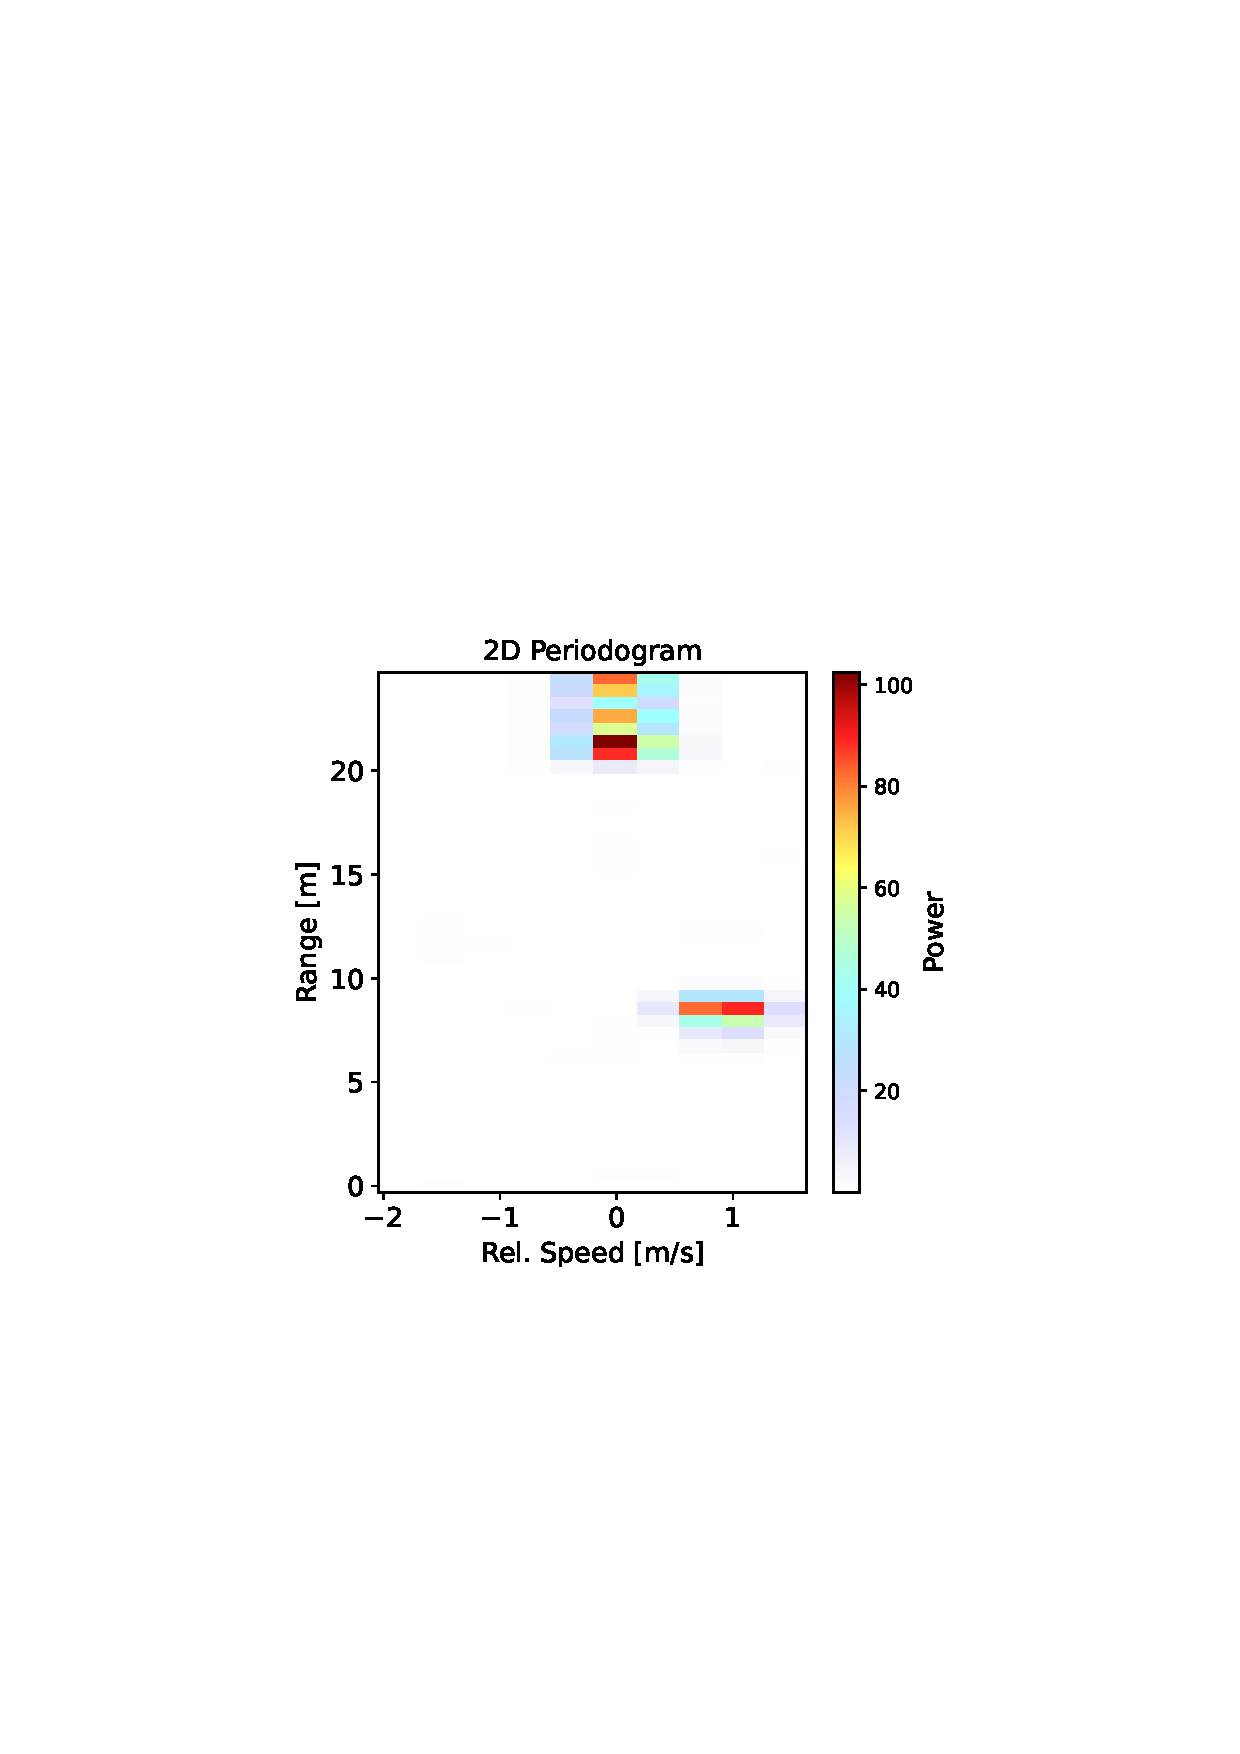
\includegraphics[scale=0.4]{Images/radar_detect_threshold/clutter/crap_ecac_mov/clutter_baseline_mov1.png}%
	}\hfill
	\subfloat[\footnotesize clutter removal with \newline ECA-C, moving target.\label{fig:Rad_crap_ecac_ECAC_mov}]{%
		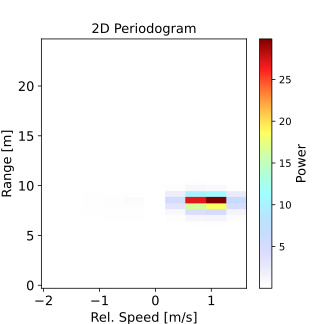
\includegraphics[scale=0.4]{Images/radar_detect_threshold/clutter/crap_ecac_mov/clutter_ecac_mov1.png}%
	}\hfill
	\subfloat[\footnotesize clutter removal using \newline CRAP, moving target. \label{fig:Rad_crap_ecac_CRAP_mov}]{%
		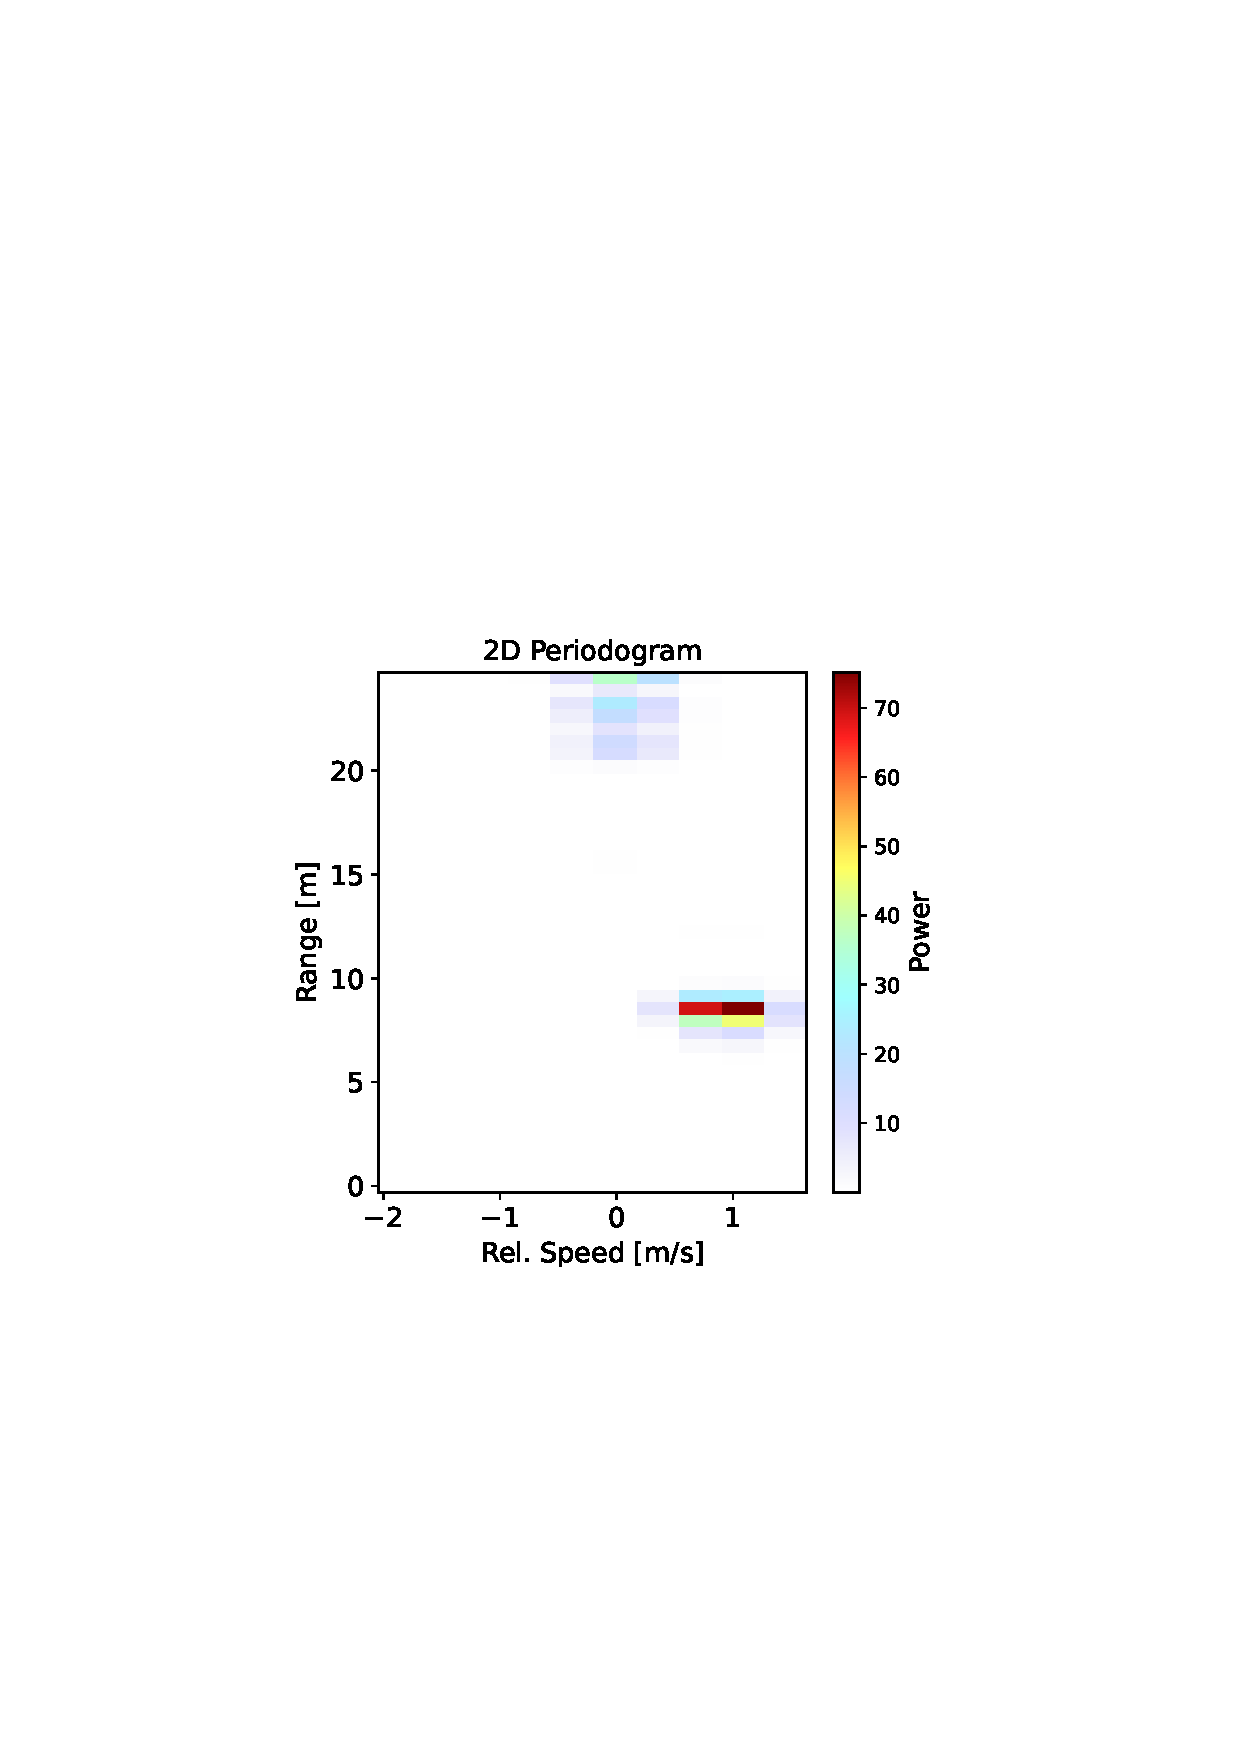
\includegraphics[scale=0.4]{Images/radar_detect_threshold/clutter/crap_ecac_mov/clutter_crap_mov1.png}%
	}
	\caption[]{\small Comparison of periodograms from sensing acquisitions obtained in NOKIA's indutrial test facility.
		Periodograms without clutter removal (left) are compared with those obtained after applying ECA-C (middle) and CRAP (right). It can be observed how ECA-C is able to clean the image from static clutter, albeit at the cost of losing information on static targets, as shown in \subref{fig:Rad_crap_ecac_ECAC_static}, whilst CRAP is able to retain the information.  }
	\label{fig:Rad_clutter_crap-ecac}
\end{figure}
\section{Clutter removal}
\label{sec:clutter_removal}

	Clutter removal in radar systems refers to the process of mitigating or eliminating unwanted signals or interference that arise from various sources (such as terrain, sea, or atmospheric conditions) and can obscure the detection of true radar targets.
	In general it is possible to refer clutter as any unwanted reflection from targets that are not of interest for the radar scope \cite{Richards_Scheer_Holm_2010}.
	
	In this work two existing implementations of clutter removal algorithms were applied to the \gls{csi} matrix.
	Both of them work by projecting the signal into a subspace orthogonal to the clutter.
	Both algoritms make use of an offline clutter acquisition step, performed before the sensing task. This step is used to gather information about clutter to be removed at runtime.
	
	\paragraph{Extensive Cancellation Algorithm by Subcarrier (ECA-C):}
	This algorithm, described in \cite{Wan_Cheng_Gong_Zhao_Shao_2012}, applies ECA \cite{Colone_ECA_2009} separately on each subcarrier of the CSI matrix.
	This approach is successful in removing the static clutter from the periodogram, at the cost of losing information on static targets and applying some distortion to targets moving at low speed.
	\paragraph{Clutter Removal with Acquisitions Under Phase Noise (CRAP):}
	CRAP introduces a novel approach by vectorizing the \gls{csi} matrices and preserving all information in both domains, unlike ECA-C which only works on each subcarrier separately and focuses solely on the time domain of the signal \cite{Henninger_CRAP_2023}.
	A detailed comparison between the two approaches can be seen in Figure \ref{fig:Rad_clutter_crap-ecac}. CRAP is able to remove static clutter without distorting the position of the target. \alert{ARGOMENTARE MEGLIO LA FIGURA}
	
	
	\subsubsection{Clutter presence in NLOS}
	
	In a \gls{nlos} sensing setup, it is fairly easy to distinguish moving targets from the underlying noise floor.
	However, static \gls{nlos} taergets cannot be easily distinguished from clutter. Static clutter in \gls{nlos} is generated by any multipath reflection of objects in the environment returning to the RX. Furthermore, these component are typically attenuated by the clutter removal algorithm.
	Figure \ref{fig:Rad_clutter_comparison} compares the appearance of a \gls{nlos} target return when the target is moving \subref{fig:Rad_clutter_mov_target} and is static \subref{fig:Rad_clutter_stat_target}.

	For \gls{nlos} intrusion detection purposes, it is sufficient to detect an intruder only when it moves, as moving targets are more likely to represent potential threats or dangerous activities. 
	Therefore, the static bins of the periodogram are discarded for \gls{nlos} processing.
	\begin{figure}[H]
		\centering
		
		\subfloat[\label{fig:Rad_clutter_mov_target}]{%
			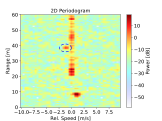
\includegraphics[scale=0.49]{Images/radar_detect_threshold/clutter/clutter_mov_target1.png}%
		}\hfill
		\subfloat[\label{fig:Rad_clutter_stat_target}]{%
			\includegraphics[scale=0.49]{Images/radar_detect_threshold/clutter/clutter_stat_target1.png}%
		}
		
		\caption[]{Periodograms with moving \subref{fig:Rad_clutter_mov_target}, and static \subref{fig:Rad_clutter_stat_target} targets in NLOS.
			Target is highlighted clearly when moving, while it appears as static clutter when it stops moving.}
		\label{fig:Rad_clutter_comparison}
	\end{figure}
	
	\section{NLOS-focused processing}
	\label{sec:nlos_proc_pipeline}
	
		\subsection{Line-of-sight and Non-line-of-sight separation}
		\label{sec:los_nlos_separation}
			
			A first necessary step for \gls{nlos} sensing is to determine which of the returns in the periodogram are generated by targets in \gls{nlos} conditions.
			It can be assumed that, in order to ensure \gls{nlos} coverage, the signal must be directed towards a large obstacle, before being reflected towards the actual target.
			Any target return with a detected range greater than that of the large obstacle can then be considered a \gls{nlos} return.
		
		
			In addition to clutter removal, calibration measurements provide valuable information for determining the distance threshold at which targets can be assumed to be in \gls{nlos}. 
			A portion of the calibration frames can be processed as radar frames, with a focus on the analysis of the zero-Doppler component.
			Figure \ref{fig:Test1_cali_static_per} depicts the sensing range information for static targets detected during calibration. 
			A target with large \gls{rcs} is detected approximately $25$ m away from the system. 
			It can be assumed that any return associated with a range greater than $25$ m is generated by a signal reflected from the largest static target.
			The figure also indicates that static clutter has a larger amplitude for ranges greater than $25$ m compared to lower ranges.
			This is due to the part of the beam that is reflected from the wall towards the environment and the associated returns.
			
			The distance between the \gls{gnb} and the reflector of the \gls{nlos} components can be estimated during the calibration step by extracting the range of the strongest static clutter component during calibration.
			
			
			\begin{figure}[H]
				\centering
				\includegraphics[width=0.6\textwidth]{Images/Test1/cali_static_per_t1.eps}
				\caption{\small Zero Doppler component of a periodogram generated from calibration measurements. It can be assumed that any returns detected beyond 25 m from the system are generated from multiple reflections and should be considered as \gls{nlos} components. }
				\label{fig:Test1_cali_static_per}
			\end{figure}
		
	
		\subsection{Modified periodogram}
			
			From the standard periodogram, considering clutter presence and the assumptions on the intrusion detection use case, regions of interest for \gls{nlos} sensing are defined.		
			Figure~\ref{fig:Rad_nlos_los_separation} highlights the regions of interest within the periodogram.
			The red area, which corresponds to static targets, is discarded. The periodogram is then divided horizontally into two regions, based on the range of the reflector for \gls{nlos}.
			
			\begin{figure}[H]
				\centering
				\includegraphics[width=1.1\textwidth]{Images/Test1/nlos-los-separation.png}
				\caption{\small Example of measured periodogram.
					The static return at 23 m is generated by a wall.
					The \gls{nlos} region is highlighted in blue, discarded static bins in red.}
				\label{fig:Rad_nlos_los_separation}
			\end{figure}
			
			
			After generating the periodogram, this separation is used to process the \gls{nlos} section and \gls{los} section separately.
		
		\subsection{Processing of the NLOS region}
		
			After defining the two regions of interest from the periodogram and discarding the static components, as described in Section \ref{sec:los_nlos_separation}, peak detection and any additional processing can be conducted separately for each region. 
			Figure \ref{fig:Test1_NLOS-proc-pipeline} summarizes the proposed processing steps for NLOS sensing.
			
			%The chosen detection strategy was CA-CFAR, which utilized a square contribution window and a probability of false alarm $p_{\text{FA}} = 10^{-6}$. The size of the CA-CFAR window was set depending on the width of the target in speed bins, which depended on number of processed frames and OFDM sampled symbols.
			
			\begin{figure}[H]
				\centering
				\includegraphics[width=0.8\textwidth]{Images/Test1/NLOS-proc-pipeline_wide_text12.png}
				\caption{\small Periodogram processing pipeline used for detection tests.}
				\label{fig:Test1_NLOS-proc-pipeline}
			\end{figure}
			
			
		 
			
			% TODO: add info on target dimensions for CA-CFAR, human case since guard cells were set in meters
			
		









% First Measurements
\chapter{NLOS measurements results}

The CSI processing approaches and radar algorithms presented in the previous sections were evaluated with real measurements obtained using Nokia's ISAC FR2 prototype described in Section \ref{sec:intro-PoCarchitecture}.

\section{Measurements setup}
\label{sec:Test1_meas_scenario}

The system was mounted in an indoor industrial test facility, with gNB and sniffer positioned at a height of $5.12$ m. The transmitter was oriented towards a wide  indoor area free of obstacles. The antenna pole was located approximately 23 metres from a warehouse rack (installed in front of a concrete wall) and a cargo door.
Figure \ref{fig:Test1_arena_plan} shows a scheme of the test area layout.

The measurement area observed was free of any major obstructions or occlusions that could be used to create a non-line-of-sight scenario under normal conditions. 

The tests were carried out using:

\begin{enumerate}
	\item A human target.
	\item A strong reflector (large metal cabinet with flat surfaces).
\end{enumerate}

The direction (azimuth $\theta$ and elevation $\varphi$) of the transmitted beam was fixed for the whole measurement.

Before each test, a short calibration measure is performed, which includes only the static elements of the scenario. The calibration data will be used in the post-processing steps for clutter removal as described in Section \ref{sec:clutter_removal}.

\begin{figure}[H]
	\centering
	\includegraphics[width=.6\textwidth]{Images/Test1/arena_plan}
	\caption{Scheme of the PoC deployment layout in ARENA 2036, Stuttgart.}
	\label{fig:Test1_arena_plan}
\end{figure}


\begin{figure}[H]
	\centering
	\includegraphics[width=1\textwidth]{Images/Test1/base-lateral_view_los_geometry}
	\caption{\small Lateral view of measurement scenario. NLOS return (red) is coupled with a LOS component (orange) generated from the secondary lobe.
	\alert{FIX ANTENNA HEIGHT WITH DOT}}
	\label{fig:Test1_base-lateral_view}
\end{figure}

\section{Measurement Scope: Detection Rate}

The radar system using OFDM can determine the range and radial speed of a target (this experiment used a fixed beam, hence the angle of arrival (AOA) was considered constant). If an object moves azimuthally within the transmitted beam, it will appear as static to the sensing system.

The test aimed to maximize the radial speed of the target to analyse the characteristics of the signal generated by its reflection through the wall.

During the initial measurement, the antenna boresight was directed perpendicular to the wall, with null azimuth $\theta$.
The target moved radially between the transmitter and reflector. The test subject moved towards the gNB and back multiple times in a straight line during the measurements.

\begin{figure}[H]
	\centering
	\includegraphics[width=1\textwidth]{Images/Test1/base-top_view}
	\caption{\small Top view of measurement scenario.}
	\label{fig:Test1_base-top_view}
\end{figure}


The beam elevation was chosen to be as high as possible to pass over the target and reflect on the wall, simulating a non-line-of-sight (NLOS) environment.

Due to the rather large beamwidth of the system, $\pm$7\textdegree\hspace{1pt} in azimuth and elevation, and its sidelobes, the measurement observed the presence of a LOS target return in addition to the expected NLOS one generated by reflection.

During the measurement, the direct component was always visible as no other obstacle was positioned in the scene. It was then decided to use the LOS return and the knowledge of the geometry of the test area to obtain an estimate of the position and velocity of the NLOS return. 
The direct target return provided additional information, which was then used as ground truth to determine the correct position of the person within the test area.
Figures \ref{fig:Test1_base-lateral_view} and \ref{fig:Test1_base-top_view} depict a scheme of the measurement.

Considering the processing scheme proposed in Section \ref{sec:nlos_proc_pipeline}, the periodogram was processed differently after separation in the regions corresponding to LOS and NLOS conditions.
A standard strongest peak search was performed for the LOS region, while multiple peak detection was conducted in NLOS, where only the five strongest peaks were considered. This assumption was made since the test was conducted in a single target scenario and a single NLOS return is expected.
Accurate range and velocity measurements are obtained after interpolation of each peak with the adjacent bins.

\begin{itemize}
	\item Speed of the NLOS component was estimated as:
	$$ \hat{v}_{\text{NLOS}} = -v_{\text{LOS}}$$
	since the direct and reflected beams will hit the target from the opposite direction, hence measuring the target's speed with opposing sign.
	\item Range of the NLOS component was estimated considering the model in Figure \ref{fig:Test1_base-lateral_view} as:
	$$ \hat{d}_{\text{NLOS}} = 2 d_{\text{wall}} - d_{\text{LOS}}\cdot \cos{(\arctan{\left(\frac{h_{\text{gNB}}}{d_{\text{LOS}}}\right)})}$$
\end{itemize}


\textit{Detection rate} was defined as the metric used to evaluate the experiment: if the speed and range of the NLOS return matched the expected values calculated from the LOS data, detection was considered positive.
The detection rate was then obtained as the ratio between the number of frames in which the NLOS component was above threshold, and the total number of frames in which the LOS component was detected.


\begin{equation*}
	\text{Detection rate} = \frac{\text{frames with NLOS}}{\text{frames with LOS}}
\end{equation*}

Due to the multiple reflections, the NLOS return presented considerably smaller power compared to LOS.
This meant that due to the presence of large clutter returns and their sidelobes, this return is not necessarily the strongest one in the NLOS region of the periodogram.
Detection rate was hence evaluated comparing the five strongest returns in NLOS with the estimated position of the target.


\section{Observation on detection rate of a strong reflector}

	\begin{figure}[H]
	\centering
	
	\subfloat[\footnotesize Metal cabinet moving towards gNB, linear scale.\label{fig:Test1_metal_lin}]{%
		\includegraphics[scale=0.45]{Images/Test1/per_strong_ref/linear_1frame_dec_CRAP.png}%
	}\hfill
	\subfloat[\footnotesize Metal cabinet moving towards gNB, power in dB.\label{fig:Test1_metal_db}]{%
		\includegraphics[scale=0.45]{Images/Test1/per_strong_ref/db_1frame_dec_CRAP_labelled_text22.png}%
	}\hfill
	\subfloat[\footnotesize Human target walking towards gNB, power in dB.\label{fig:Test1_metal_human-baseline}]{
		\includegraphics[scale=0.45]{Images/Test1/per_strong_ref/db_1frame_dec_CRAP_HUMAN_labelled_text22.png}
	}
	\caption[]{\small Comparison of periodograms from sensing acquisitions obtained in NOKIA's industrial test facility.
		All the periodograms are obtained by processing a single decimated CSI frame (24 symbols), after applying clutter removal with CRAP.
		Periodograms \subref{fig:Test1_metal_lin} and \subref{fig:Test1_metal_db} show the returns obtained with the metal cabinet. The NLOS return (purple) is clearly separated from the underlying noise floor, even when processing only 24 symbols. On the contrary the NLOS component generated from the human target in \subref{fig:Test1_metal_human-baseline}, requires for a considerably higher processing gain to be detected reliably.}
	\label{fig:Test1_metal-human_comparison}
	\end{figure}
	
The first measurement was performed with the strong reflector, which represented an ideal scenario. 
Figure \ref{fig:Test1_metal-human_comparison} illustrates the comparison between the human and the metal cabinet cases. 
Even when decimating the single CSI matrix, with a 15 dB loss in processing gain, the NLOS component of the metal cabinet can be easily identified when moving.

The detection rate test displayed in figure \ref{fig:Test1_detect_rate_strong_ref} shows that the passive reflector, thanks to its significantly larger radar cross section, is clearly identified while it is moving and has stronger power compared to reflected clutter returns.

Passing the NLOS measurements to a Kalman filter it was possible to track the target in the range/Doppler plane, as shown in figure \ref{fig:Test1_kf_track_strong_ref}. This result is to show that one of the main limitation of NLOS signals is the strength of the target return. Objects with large RCS are easier to separate from the noisy background and the effect of fading and obstruction is relatively small.

\begin{figure}[H]
	\centering
	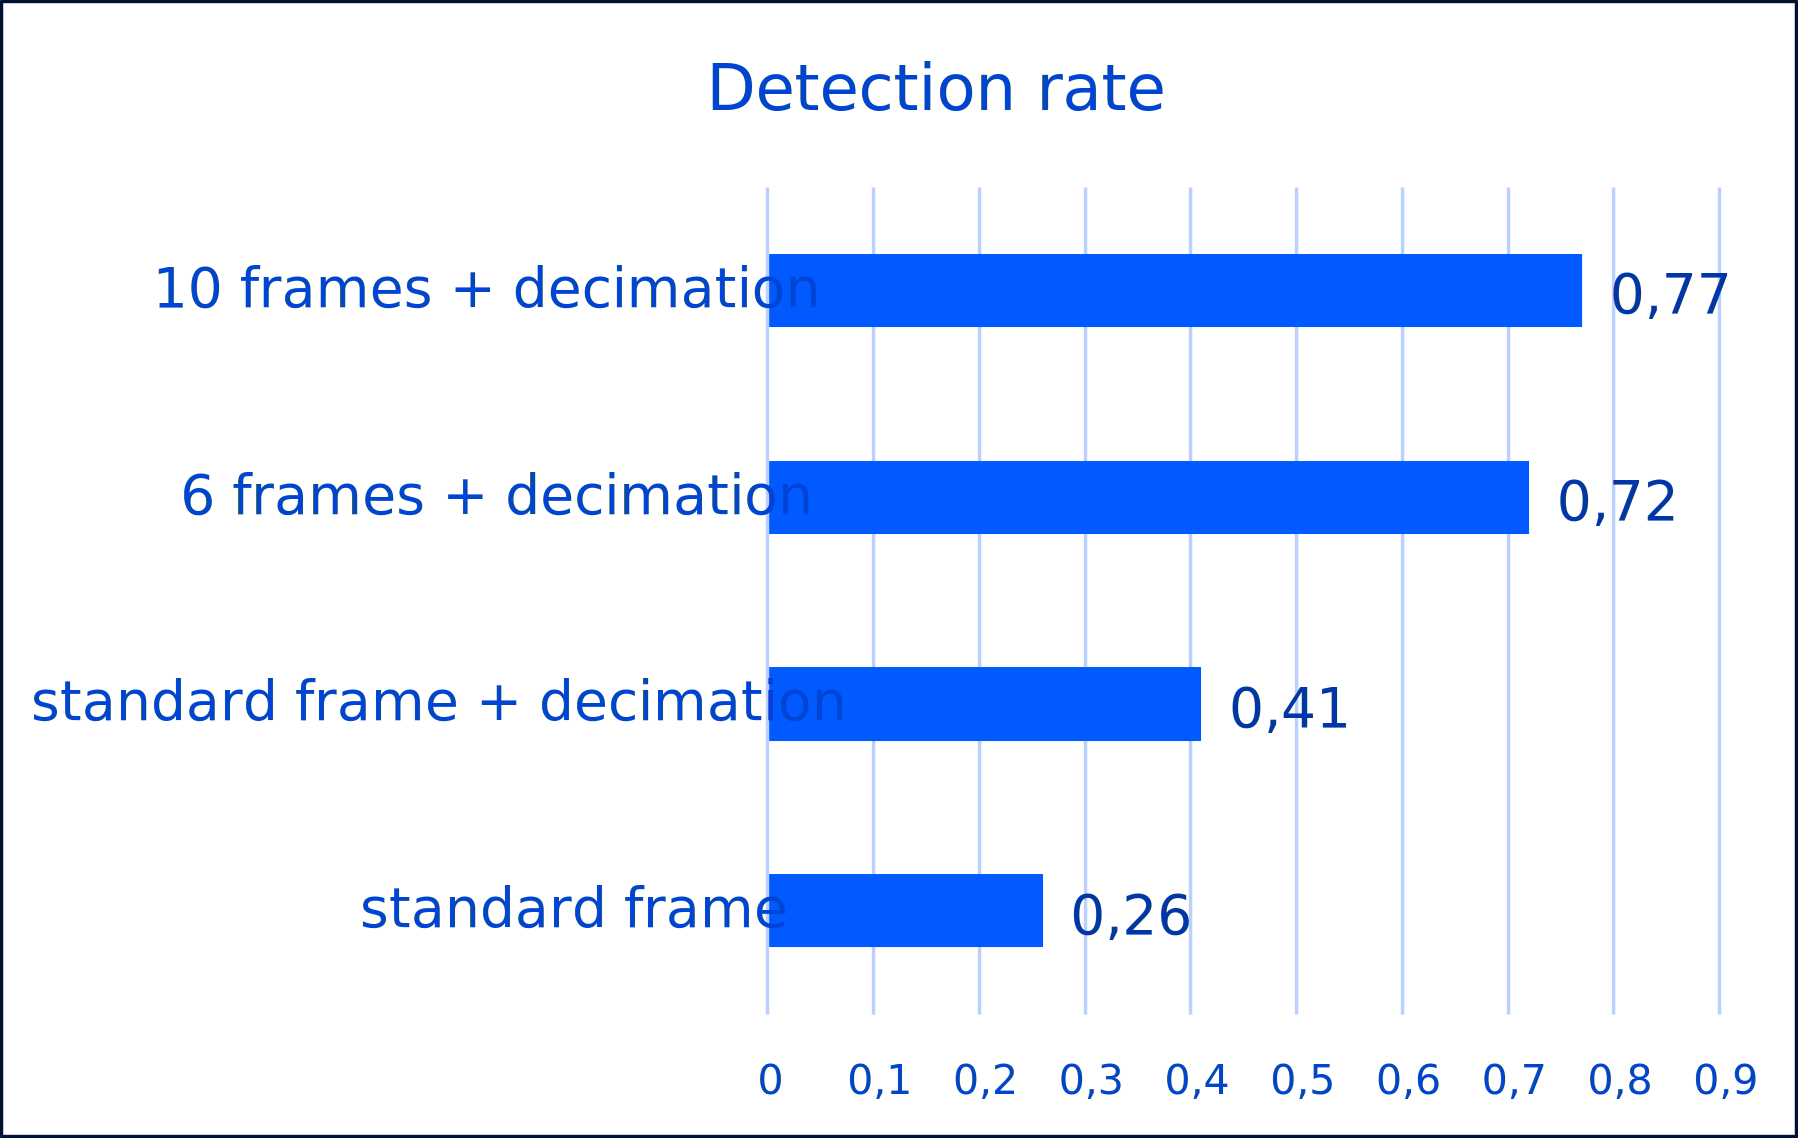
\includegraphics[width=0.55\textwidth]{Images/Test1/detect_hist/detect_hist_cabinet_LMsans.png}
	\caption{\small Detection rate observed for passive metal reflector target in mixed LOS/NLOS measurement.}
	\label{fig:Test1_detect_rate_strong_ref}
\end{figure}



\begin{figure}[H]
	\centering
	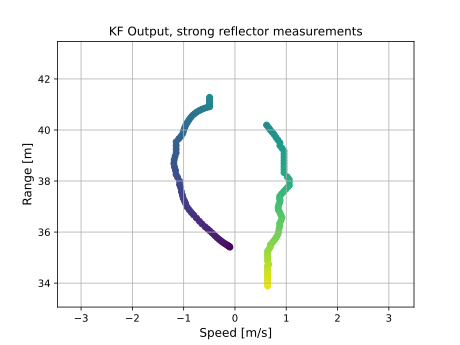
\includegraphics[width=0.55\textwidth]{Images/Test1/kf_track.eps}
	\caption{\small KF track of the target in the range/speed plane. Track is interrupted when the target stops and changes direction.}
	\label{fig:Test1_kf_track_strong_ref}
\end{figure}


\subsection{Human target detection}

The detection rate for measurements with a walking actor was obtained using the various frame processing strategies presented in chapter \ref{chap:TDD pattern of the OFDM frame}. To increase time-aperture, subsequent frames were combined, and the window processing stride was set to be lower than the number 
of frames, allowing for more target updates.

Clutter removal was performed using CRAP to ensure precise estimation of the expected target position in NLOS conditions. In contrast, periodograms generated with the ECA-C technique showed the NLOS component to be well separated from the underlying noise floor, but the estimated position did not correspond with the measured one, making the detection test difficult. Comparison of a sample radar update after CRAP and ECA-C is shown in Figure \ref{fig:Test1_huma_crap-ecac}.

	\begin{figure}[H]
	\centering
	
	\subfloat[Periodogram after applying CRAP.\label{fig:Test1_mhuman_crap}]{%
		\includegraphics[scale=0.45]{Images/Test1/Human_crap_ecac/crap_labelled.png}%
	}\hfill
	\subfloat[Periodogram after applying ECA-C.\label{fig:Test1_mhuman_ecac}]{%
		\includegraphics[scale=0.45]{Images/Test1/Human_crap_ecac/ecac_labelled.png}%
	}
	\caption[]{\small Comparison of periodograms from sensing acquisitions obtained in NOKIA's industrial test facility.
		Periodogram obtained by processing 6 consecutive frames.
		In \subref{fig:Test1_mhuman_crap} the NLOS return presents a single, but its power is comparable with the one of the nearby artefacts. In \subref{fig:Test1_mhuman_ecac} the return is distorted in two peaks, moreover the sidelobes of the LOS component are enhanced and appear as ghost targets.}
	\label{fig:Test1_huma_crap-ecac}
\end{figure}




Target detection was carried out by considering the \textit{n}-strongest peaks and comparing them against the LOS data. If any of the observed non-line-of-sight (NLOS) peaks corresponded to the target, then the detection was positive.

\begin{figure}[H]
	\centering
	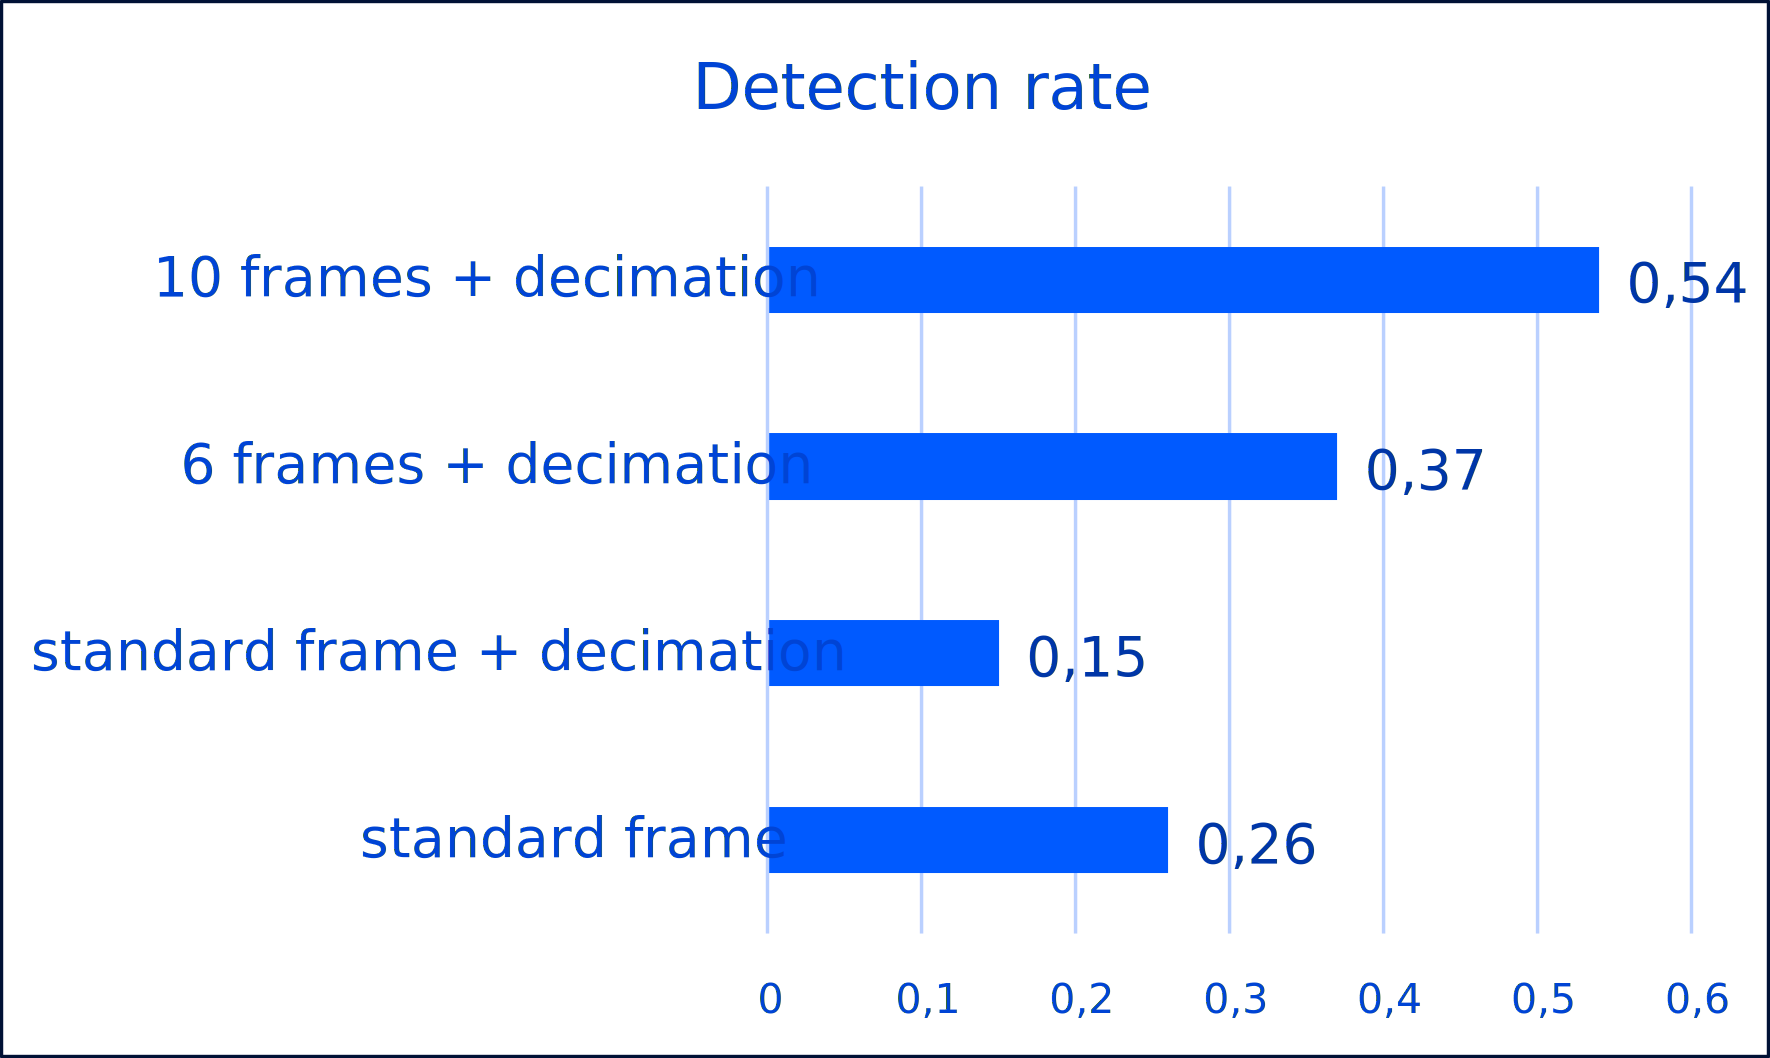
\includegraphics[width=0.7\textwidth]{Images/Test1/detect_hist/detect_hist_human_LMsans.png}
	\caption{Detection rate observed for human target in mixed LOS/NLOS measurement. Clutter removal performed with CRAP.}
	\label{fig:Test1_detect_hist}
\end{figure}

Increasing the time-aperture significantly improved the detection rate due to the larger SNR.

In most cases, the NLOS target return was not the strongest due to lower peak power compared to noise. Additionally, when increasing the time aperture, spectral artefacts were present.
Target returns occasionally suffered from channel fading, causing their power to change between consecutive updates. In contrast, artefacts' power remained relatively constant and proportional to the number of processed frames.

The detection rate was observed throughout the entire measurement, including frames where the target changed direction and was either static or presented a low-speed component. However, processing these time instants may have masked the NLOS component with clutter and resulted in a negative detection. Therefore, the effective detection rate, which is measured only when the target is in motion, is likely to be higher.


%TODO: change subsection title
\subsubsection{Moving average of detection rate}

Figure \ref{fig:Test1_moving_avg} shows the average detection rate over 10 consecutive updates. It is evident that the detection rate is above 80\% for several consecutive 10-update intervals when the target is in motion and therefore well separated from the clutter region.


Although this measure was obtained in a controlled single-target scenario, it opens the possibility of detecting the presence of non-line-of-sight (NLOS) moving targets without relying on additional ground truth data.


% TODO: change picture with higher resolution one, maybe solved
\begin{figure}[H]
	\centering
	\includegraphics[width=0.7\textwidth]{Images/Test1/moving_avg-transformed_wtext}
	\caption{Detection rate observed for human target in mixed LOS/NLOS measurement.}
	\label{fig:Test1_moving_avg}
\end{figure}


\subsubsection{Detection rate with separate clutter removal for NLOS}

Figure \ref{fig:Test1_huma_crap-ecac} illustrates the tradeoffs between using CRAP and ECA-C for clutter removal. It can be seen that CRAP is ideal for line-of-sight (LOS) targets, while the power of the non-line-of-sight (NLOS) return is reduced to a level similar to the Doppler artefacts.

On the other hand, ECA-C introduces distortion and loss of information at zero speed, which is not suitable for any use case requiring LOS. In NLOS the static bin of the periodogram is discarded anyway, while the target return can be easily distinguished from the underlying noise floor.

The detection rate was tested using CRAP and ECA-C for the LOS and NLOS regions respectively, and the results are shown in Figure \ref{fig:Test1_moving_avg}.
This approach improved detection when the target was in motion.

\begin{figure}[H]
	\centering
	\includegraphics[width=0.7\textwidth]{Images/Test1/detect_hist/detect_hist_human_ECAC_LMsans.png}
	\caption{\small Detection rate observed for human target in mixed LOS/NLOS measurement. Clutter removal performed with ECA-C for the NLOS region and CRAP for the LOS.}
	\label{fig:Test1_detect_hist_crap-ecac}
\end{figure}


The measurement was not affected by the loss of information due to ECA-C when the target was static, as the bins of the periodogram corresponding to null speed were discarded regardless.

The moving average of the detection probability is shown in Figure \ref{fig:Test1_mov_avg_crap_ecac}.
It is evident that the detection from seconds 5 to 7 is significantly improved when compared to using only CRAP.
However, this approach incurs a high computational cost as both clutter removal methods need to be applied to each OFDM frame separately.

\begin{figure}[H]
	\centering
	\includegraphics[width=0.8\textwidth]{Images/Test1/ECAC_CRAP_mixed/movavg_6frames_mixedecac-crap_stride4_exp_thresh.png}
	\caption{\small Detection rate observed for human target in mixed LOS/NLOS measurement. Clutter removal performed with ECA-C for the NLOS region and CRAP for the LOS.}
	\label{fig:Test1_mov_avg_crap_ecac}
\end{figure}


\chapter{Outlook and Conclusion}

This thesis investigated the integration of sensing and communication capabilities in the context of 5G Advanced and 6G wireless systems. 
The main objective of this work was to explore the potential of \gls{nlos} sensing techniques and their applications in integrated radar systems at mmWave. 

The results obtained from processing real-word measurements suggest that use cases with NLOS conditions should be considered in future studies in ISAC.
With a focus on intrusion detection this work suggests that, with further analysis of the NLOS radar returns and the corresponding processing techniques, NLOS sensing at mmWave is possible.

The main contributions of this work can be summarized as follows:

\begin{itemize}
	\item Real-word NLOS sensing trials and identification of challenges due to communication requirements.
	\item Proposal of \gls{csi} processing approaches for avoiding unwanted replicas in the periodogram.
	\item Definition of requirements for NLOS sensing and validation on measurements from the prototype.
\end{itemize}

This investigations on \gls{nlos} \gls{isac} for intrusion detection use cases only represent an introductory study on the matter.
Follow-up investigations will be required to fully explore new solutions and exploit the capabilities of the system in different scenarios.


%-------------------------------------------------------------------------
%	BIBLIOGRAPHY
%-------------------------------------------------------------------------

\addtocontents{toc}{\vspace{2em}} % Add a gap in the Contents, for aesthetics
% \bibliographystyle{IEEEtran}
\bibliography{Thesis_bibliography} % The references information are stored in the file named "Thesis_bibliography.bib"

%-------------------------------------------------------------------------
%	APPENDICES
%-------------------------------------------------------------------------

\cleardoublepage
\addtocontents{toc}{\vspace{2em}} % Add a gap in the Contents, for aesthetics
%\appendix
% \chapter{Appendix A}
%If you need to include an appendix to support the research in your thesis, you can place it at the end of the manuscript.
%An appendix contains supplementary material (figures, tables, data, codes, mathematical proofs, surveys, \dots)
% which supplement the main results contained in the previous chapters.


% ABBREVIATIONS
\glsaddall
\printglossaries[type=\acronymtype,title=Acronyms]

% LIST OF FIGURES
\listoffigures

% LIST OF TABLES
\listoftables

% LIST OF SYMBOLS
% Write out the List of Symbols in this page
\chapter*{List of Symbols} % You have to include a chapter for your list of symbols (
\begin{table}[H]
    \centering
    \begin{tabular}{lll}
        \textbf{Variable} & \textbf{Description} & \textbf{SI unit} \\\hline\\[-9px]
        $\bm{u}$ & solid displacement & m \\[2px]
        $\bm{u}_f$ & fluid displacement & m \\[2px]
        $\bm{c}_0$ & speed of light & m/s \\[2px]
        $\bm{f}_C$ & carrier frequency & Hz \\[2px]
    \end{tabular}
\end{table}

% ACKNOWLEDGEMENTS
\chapter*{Acknowledgements}
Here you might want to acknowledge someone.

\cleardoublepage


\end{document}